\documentclass[10pt]{article}

\usepackage[english]{babel}
\usepackage{placeins}
\usepackage[letterpaper,top=2.05cm,bottom=2.05cm,left=2.45cm,right=2.45cm]{geometry}
\usepackage{amsmath,amssymb}
\usepackage{graphicx}
\usepackage[colorlinks=true,linkcolor=blue!60!black,citecolor=blue!60!black,urlcolor=blue!60!black]{hyperref}
\usepackage{xurl}
\usepackage{booktabs}
\usepackage{tabularx}
\usepackage{array}
\usepackage{microtype}
\usepackage{setspace}
\usepackage[table]{xcolor}
\onehalfspacing
\emergencystretch=3em
\urlstyle{tt}

\title{\Large\bfseries Chemical lateralization in the adult fly mushroom body links structure, CyberFly propagation, and memory-circuit validation}
\author{}
\date{}

\begin{document}
\maketitle
\thispagestyle{empty}

% 中文注释：摘要先把故事讲清楚，不再从拓扑表示学习开场，而是从“左右蘑菇体是否使用不同递质”这个生物问题开场。
\begin{abstract}
The adult \textit{Drosophila} mushroom body is widely treated as a bilateral memory circuit, yet it has remained unclear whether the two hemispheres use the same transmitter logic. Here we show that Kenyon-cell (KC) inputs in FlyWire v783 are chemically lateralized rather than merely structurally asymmetric. Across 11 KC types, serotonin-predicted input is right-enriched in all types, whereas glutamate-predicted input is left-biased in 7 of 11 types, with the strongest effects in the memory-consolidation $\alpha'\beta'$ lobe. This asymmetry is not explained by KC output identity, because KC outputs are uniformly cholinergic. Sparse GPU propagation through a CyberFly-style connectome bridge shows that transmitter-selected KC ensembles do not behave like matched random controls: right-serotonin and left-glutamate seed sets recruit distinct memory-axis, DAN, APL, DPM and MBON/MBIN readouts, and direct FlyWire mining reveals a left-biased KC--APL--DPM feedback module alongside a weaker right-biased DAN--MBON axis. We then convert these readouts into wet-lab-ready hypotheses. A public DPM optogenetic surrogate prioritizes red-shifted CsChrimson/ReaChR protocols and predicts a right-biased 5-HT readout under brain-side registration. A separate OCT/MCH behavioural surrogate identifies the weak-OCT/strong-MCH conflict assay as the most sensitive group-level test. The manuscript therefore does not claim that the connectome alone generates full fly behaviour. Instead, it provides a falsifiable route from transmitter lateralization to function and validation.
\end{abstract}

% 中文注释：引言要把动机说成“结构侧化是否真的有功能意义”，同时说明我们为什么需要仿真和视频，而不只是统计表。
\section*{Introduction}
Brain lateralization is a general organizational principle, but its chemical basis is often hidden if one only counts synapses. The adult fly mushroom body (MB) is a strong place to ask this question because it is the canonical centre for associative learning, and its output is shaped by dopamine, serotonin and recurrent feedback circuits that determine how memory is written and stabilized\cite{aso2014mushroom,modi2020dopamine_kc,keene2006dpm,waddell2013serotonin}. At the same time, connectome-scale studies have repeatedly shown that bilateral differences in insects are not random noise but a reproducible feature of circuit architecture\cite{scheffer2020hemibrain,li2020kc_subtypes,karolis2019lateralisation,pedigo2023bilateral_elife,winding2023larva}. From the algorithm side, our analysis sits in a line of graph representation learning that includes DeepWalk, node2vec, LINE, GraphSAGE, graph attention networks and relational GCNs, together with topology-preserving methods such as Topological Autoencoders and PersLay\cite{deepwalk2014,node2vec2016,line2015,graphsage2017,gcn2017,gat2018,rgcn2018,topoautoenc2020,perslay2020}. For neuronal morphology, NBLAST remains a canonical reference for structure-based cell comparison\cite{costa2016nblast}.

Our question is narrower than a full embodied-brain claim: does the adult fly MB contain a reproducible transmitter-level left--right bias, and can that bias be pushed forward into experimentally useful predictions? We answer this by combining three layers. First, the structural layer asks whether the KC input transmitter profile is lateralized. Second, the propagation layer asks whether transmitter-selected KC ensembles recruit distinct memory-related readouts when they are run through a public connectome bridge. Third, the validation layer asks whether the same structural logic suggests DPM optogenetic and OCT/MCH assays that a wet lab can actually run.

% 中文注释：这里用最少的术语给非生物背景读者做底层解释，避免后面每次出现 KC/DPM/MBON 时都要回头猜。
\subsection*{Key terms in plain language}
\begin{table}[!ht]
\centering\small
\caption{\textbf{Key biological terms used in this manuscript.}}
\label{tab:terms}
\begin{tabularx}{\linewidth}{@{}p{3.2cm}X@{}}
\toprule
Term & Meaning in this paper \\
\midrule
KC & Kenyon cell, the main mushroom-body neuron class that encodes odours sparsely. \\
$\alpha'\beta'$ lobe & KC subregion linked to memory consolidation; it shows the strongest lateralization here. \\
Serotonin / 5-HT & Modulatory transmitter class. We report a right-enriched input bias. \\
Glutamate / Glu & Excitatory transmitter class. We report a left-biased input pattern in most KC types. \\
MBON & Mushroom-body output neuron, a downstream readout of memory state. \\
DAN & Dopaminergic neuron, a teaching/modulatory neuron class. \\
DPM & Mushroom-body feedback neuron that is especially relevant for memory consolidation and 5-HT readout. \\
CS+ / CS- & Conditioned stimulus paired with reinforcement / control stimulus without reinforcement. \\
OCT / MCH & 3-octanol / 4-methylcyclohexanol, the two odours used in the behavioural proxy tasks. \\
Laterality index & $(R-L)/(R+L)$, a signed measure of right-versus-left bias. \\
\bottomrule
\end{tabularx}
\end{table}

% 中文注释：Figure 1 用来把“我们到底做了什么”一次讲清楚。不要再放太多拓扑细节，这里只保留结构->传播->验证主链。
\begin{figure}[!ht]
\centering
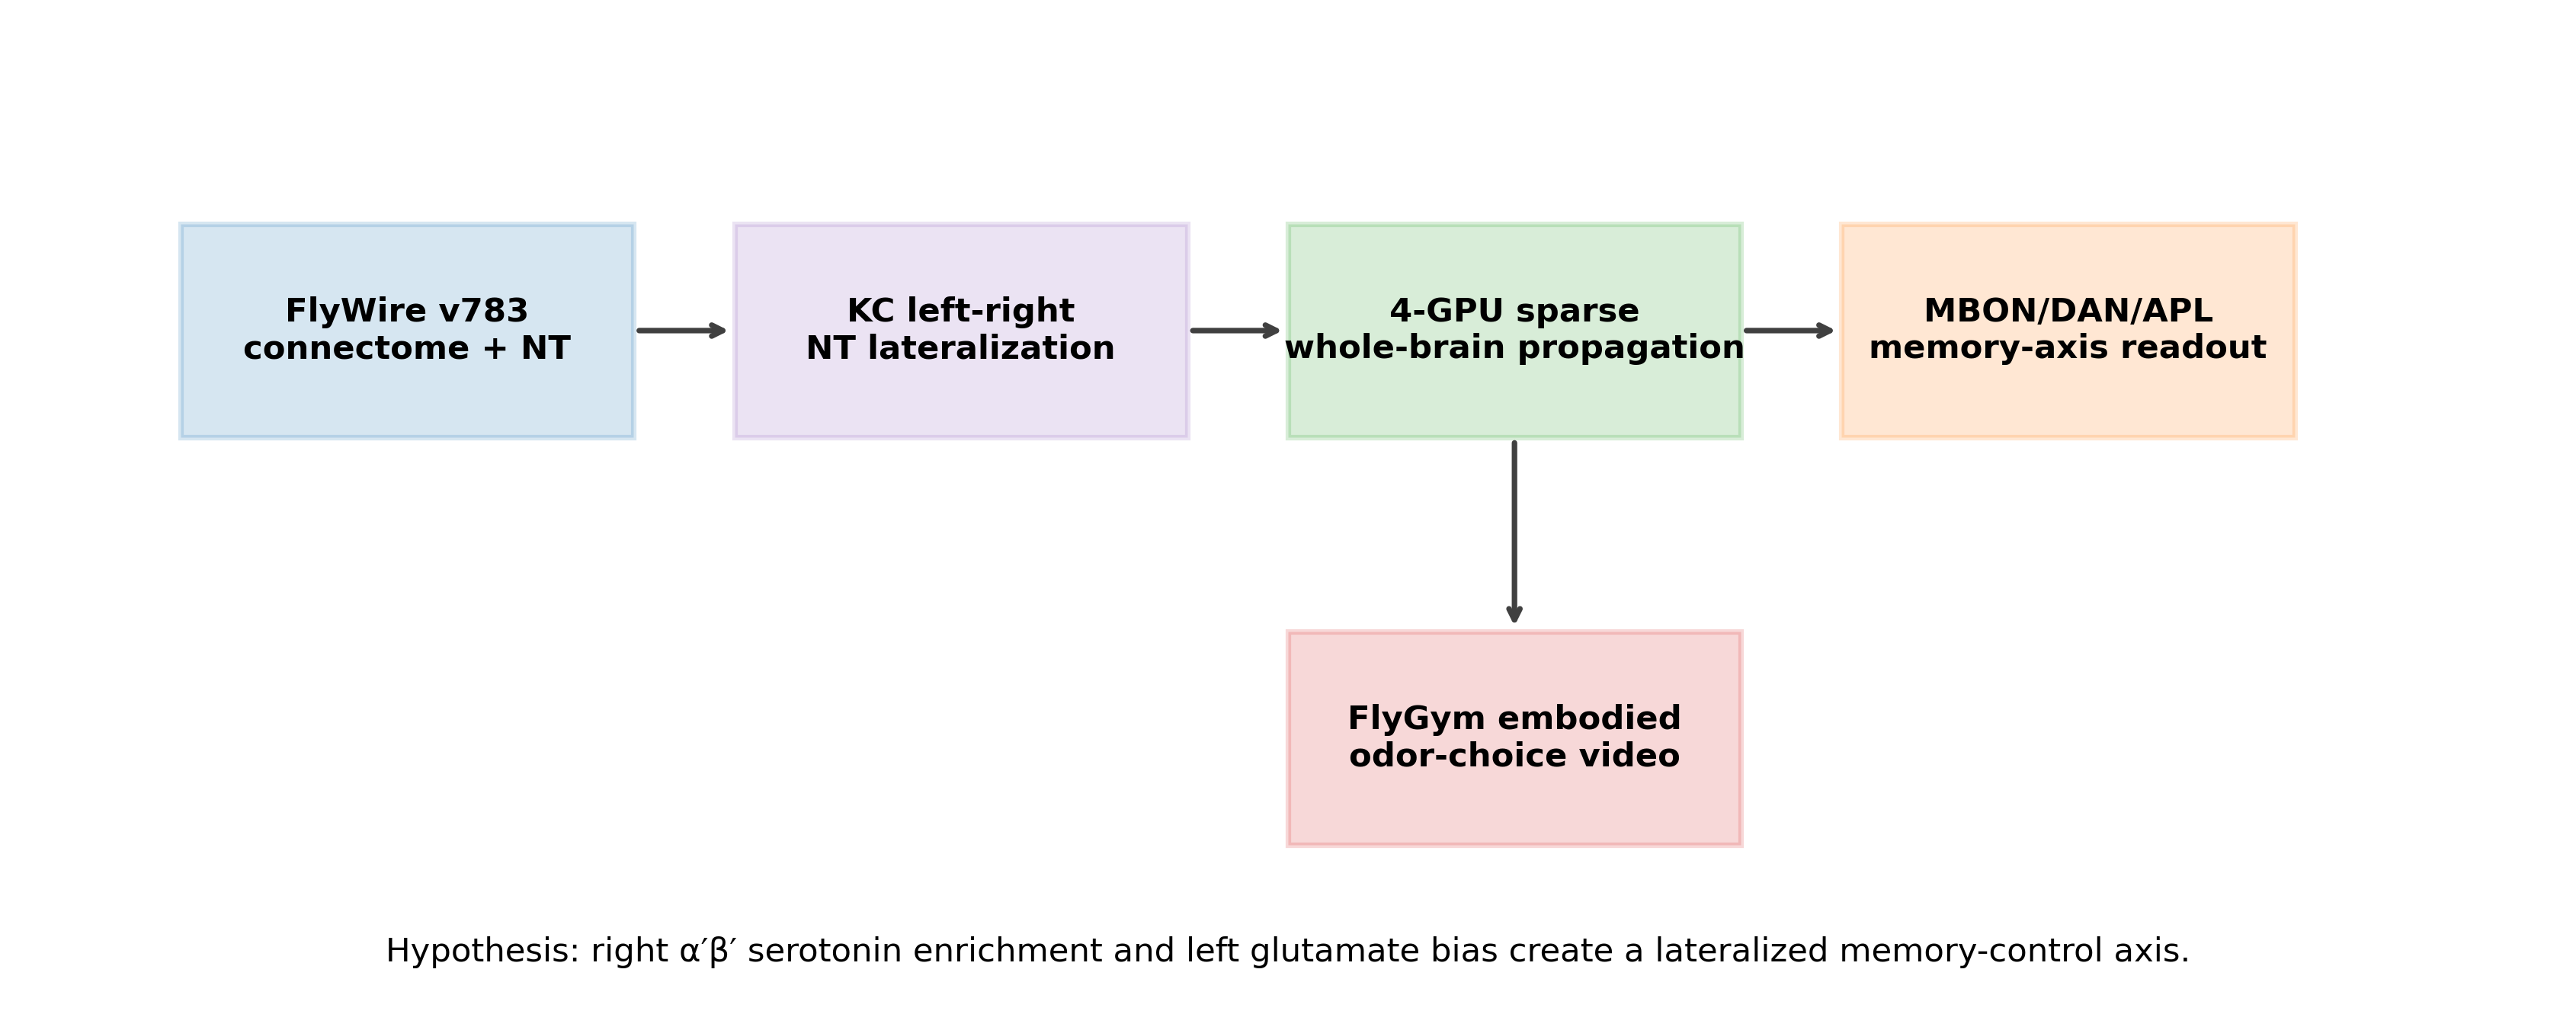
\includegraphics[width=0.63\linewidth]{figures/Fig1_cyber_fly_pipeline_mechanism.png}
\vspace{0.35em}
\includegraphics[width=0.87\linewidth]{figures/Fig0_story_and_validation.pdf}
\caption{\textbf{Study logic and CyberFly bridge.}
\textbf{a}, The public pipeline starts from FlyWire v783, then selects transmitter-defined KC seed ensembles, propagates them through the connectome, and converts the result into DPM and OCT/MCH validation hypotheses.
\textbf{b}, The same bridge separates structural discovery, functional propagation and wet-lab validation, so the paper does not over-claim that connectome alone generates full behaviour.
The supplementary video corresponding to the bridge is available at \url{/unify/ydchen/unidit/bio_fly/outputs/four_card_suite/videos/cyber_fly_lateralized_memory_axis.mp4}.}
\label{fig:story}
\end{figure}

\section*{Results}

% 中文注释：第一条结果必须是最稳的结构发现。这里直接报告右 5-HT、左 Glu、alpha'beta' 最强，并明确 KC 输出并没有变。
\subsection*{KC inputs are chemically lateralized, and the strongest bias sits in the memory-consolidation lobe}
We first asked whether KC inputs carry a stable left--right transmitter signature. Using corrected KC subtype annotations, we compared left and right KCs across 11 testable hemibrain types and six transmitter classes. The result is direct: serotonin-predicted input is right-enriched in all 11 types, while glutamate-predicted input is left-biased in 7 of 11 types. The strongest effects occur in the $\alpha'\beta'$ lobe, the KC subregion most closely linked to memory consolidation.

The effect sizes are large enough to survive multiple correction schemes. Serotonin is right-biased in 11/11 types, with 9/11 FDR-significant and 7/11 Bonferroni-significant effects. The top serotonin effects are in KCa'b'-ap2, KCa'b'-m and KCa'b'-ap1, where Cohen's $d$ reaches +1.45, +1.35 and +1.34 respectively. Glutamate shows the opposite direction in 7/11 types, is 7/11 Bonferroni-significant, and is strongest in the same $\alpha'\beta'$ types, where $d$ reaches -1.47. By contrast, KC outputs are uniformly cholinergic. The lateralization is therefore an input-side phenomenon: what changes across hemispheres is the transmitter composition that KCs receive from upstream partners, not their own output identity.

% 中文注释：Figure 2 负责把结构发现讲清楚，左边看左右差异，右边看 lobe 分层。不要再塞拓扑分类图。
\begin{figure}[!ht]
\centering
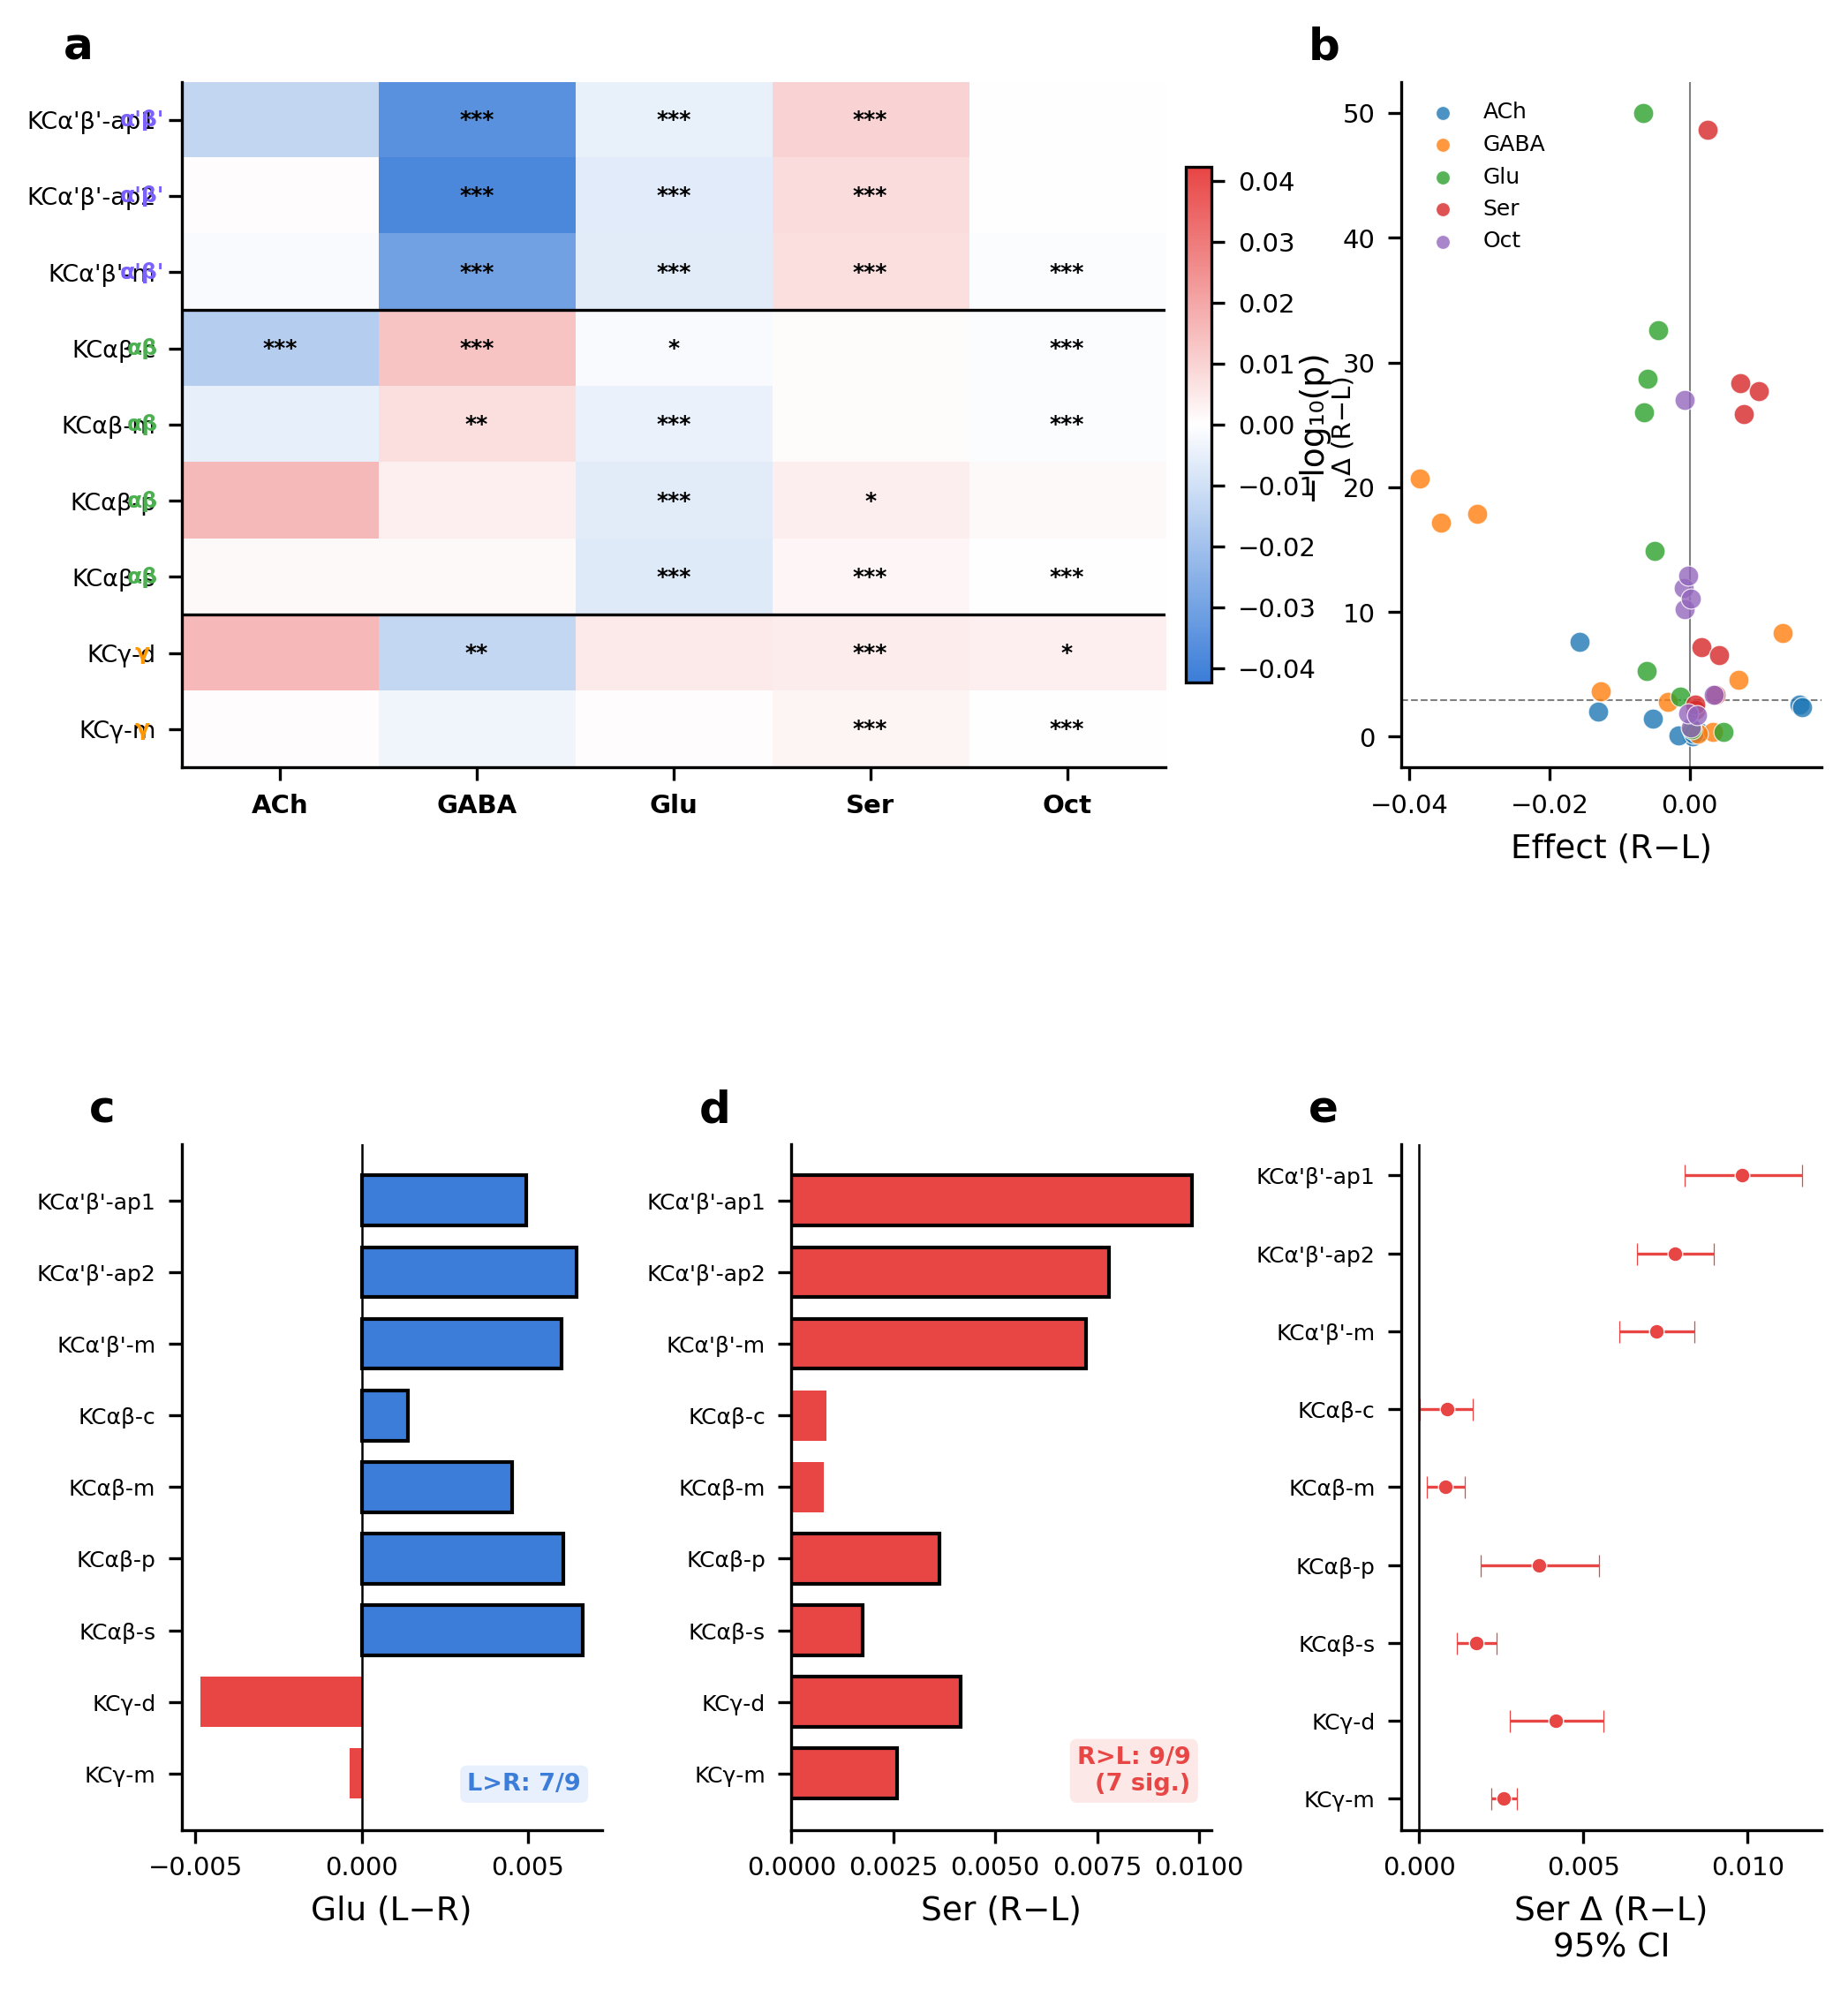
\includegraphics[width=0.49\linewidth]{figures/Fig3_hemisphere_asymmetry.png}
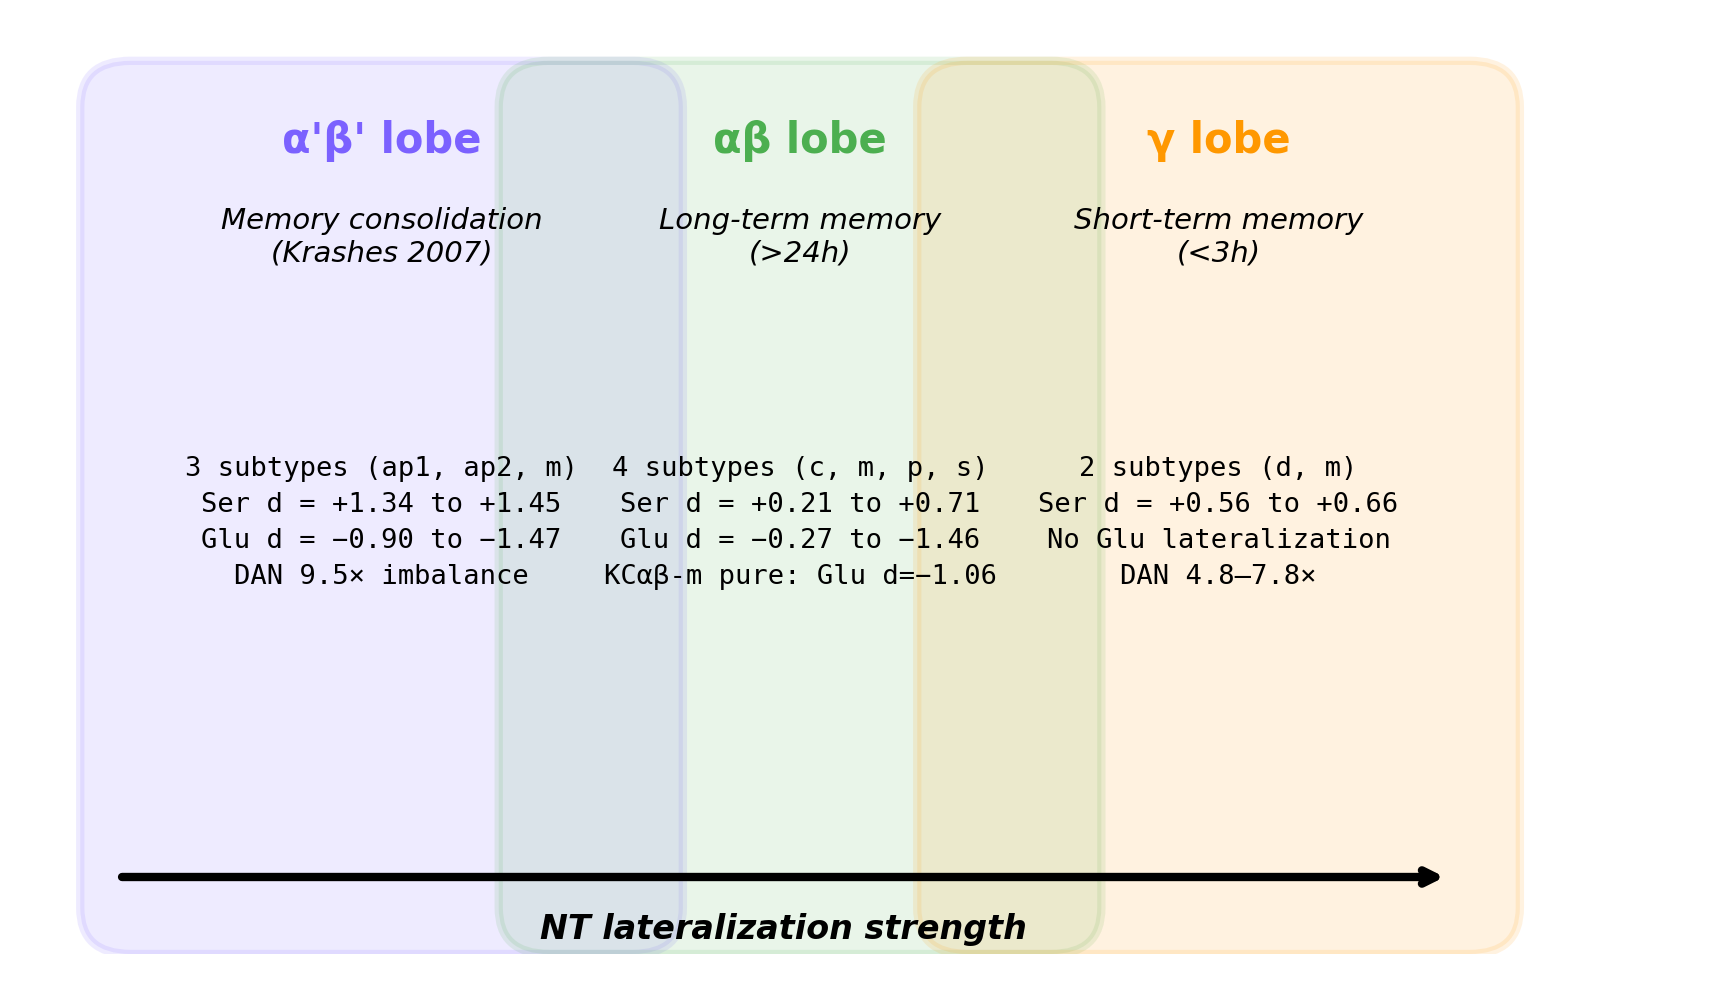
\includegraphics[width=0.49\linewidth]{figures/Fig7_lobe_memory_schematic.png}
\caption{\textbf{Structural transmitter lateralization in KCs.}
\textbf{a}, Effect-size heat map showing right-serotonin and left-glutamate biases across KC types.
\textbf{b}, Lobe-level summary showing that the strongest bias sits in the memory-consolidation $\alpha'\beta'$ subregion, with graded effects in $\alpha\beta$ and weaker effects in $\gamma$.}
\label{fig:structure}
\end{figure}

% 中文注释：第二条结果是功能传播。这里要把“不是统计表而已”讲清楚：选择性 seed 真的能把 readout 推到记忆轴和反馈轴。
\subsection*{The asymmetry propagates into memory-axis and feedback/output readouts}
Structural lateralization is only interesting if it reaches circuit-level readouts. To test that, we selected the transmitter-defined KC ensembles most clearly enriched for right-serotonin or left-glutamate input and propagated them through the FlyWire signed graph using side-matched random KC controls as nulls.

The two axes do not behave identically. Right-serotonin KC activation significantly changes DAN, APL, DPM and response laterality readouts, with FDR-corrected $q=0.038$ for the strongest metrics. Left-glutamate KC activation is broader: it significantly changes memory-axis mass, DAN, MBIN, APL, DPM, MBON and response laterality, again at FDR $q=0.038$ for the strongest metrics. This matters because it means the structural asymmetry is not a descriptive table that stops at the KC boundary. It reaches a downstream memory-related circuit geometry.

Direct mining of the MB-associated edge table supports the same interpretation. The recurrent feedback side of the circuit is left-biased: KC--APL, APL--KC, KC--DPM and DPM--KC all show leftward bias. In contrast, the modulatory/output side is weakly right-biased: DAN--MBON and MBON--DAN show a smaller but consistent rightward tendency. This suggests a division between a left-biased feedback/stabilization module and a weaker right-biased modulatory output module, rather than a single global left-right imbalance.

% 中文注释：Figure 3 应该把功能传播和靶点优先级讲成一个完整故事，一个图里说清楚“为什么这些 seed 不是随机的”。
\begin{figure}[!ht]
\centering
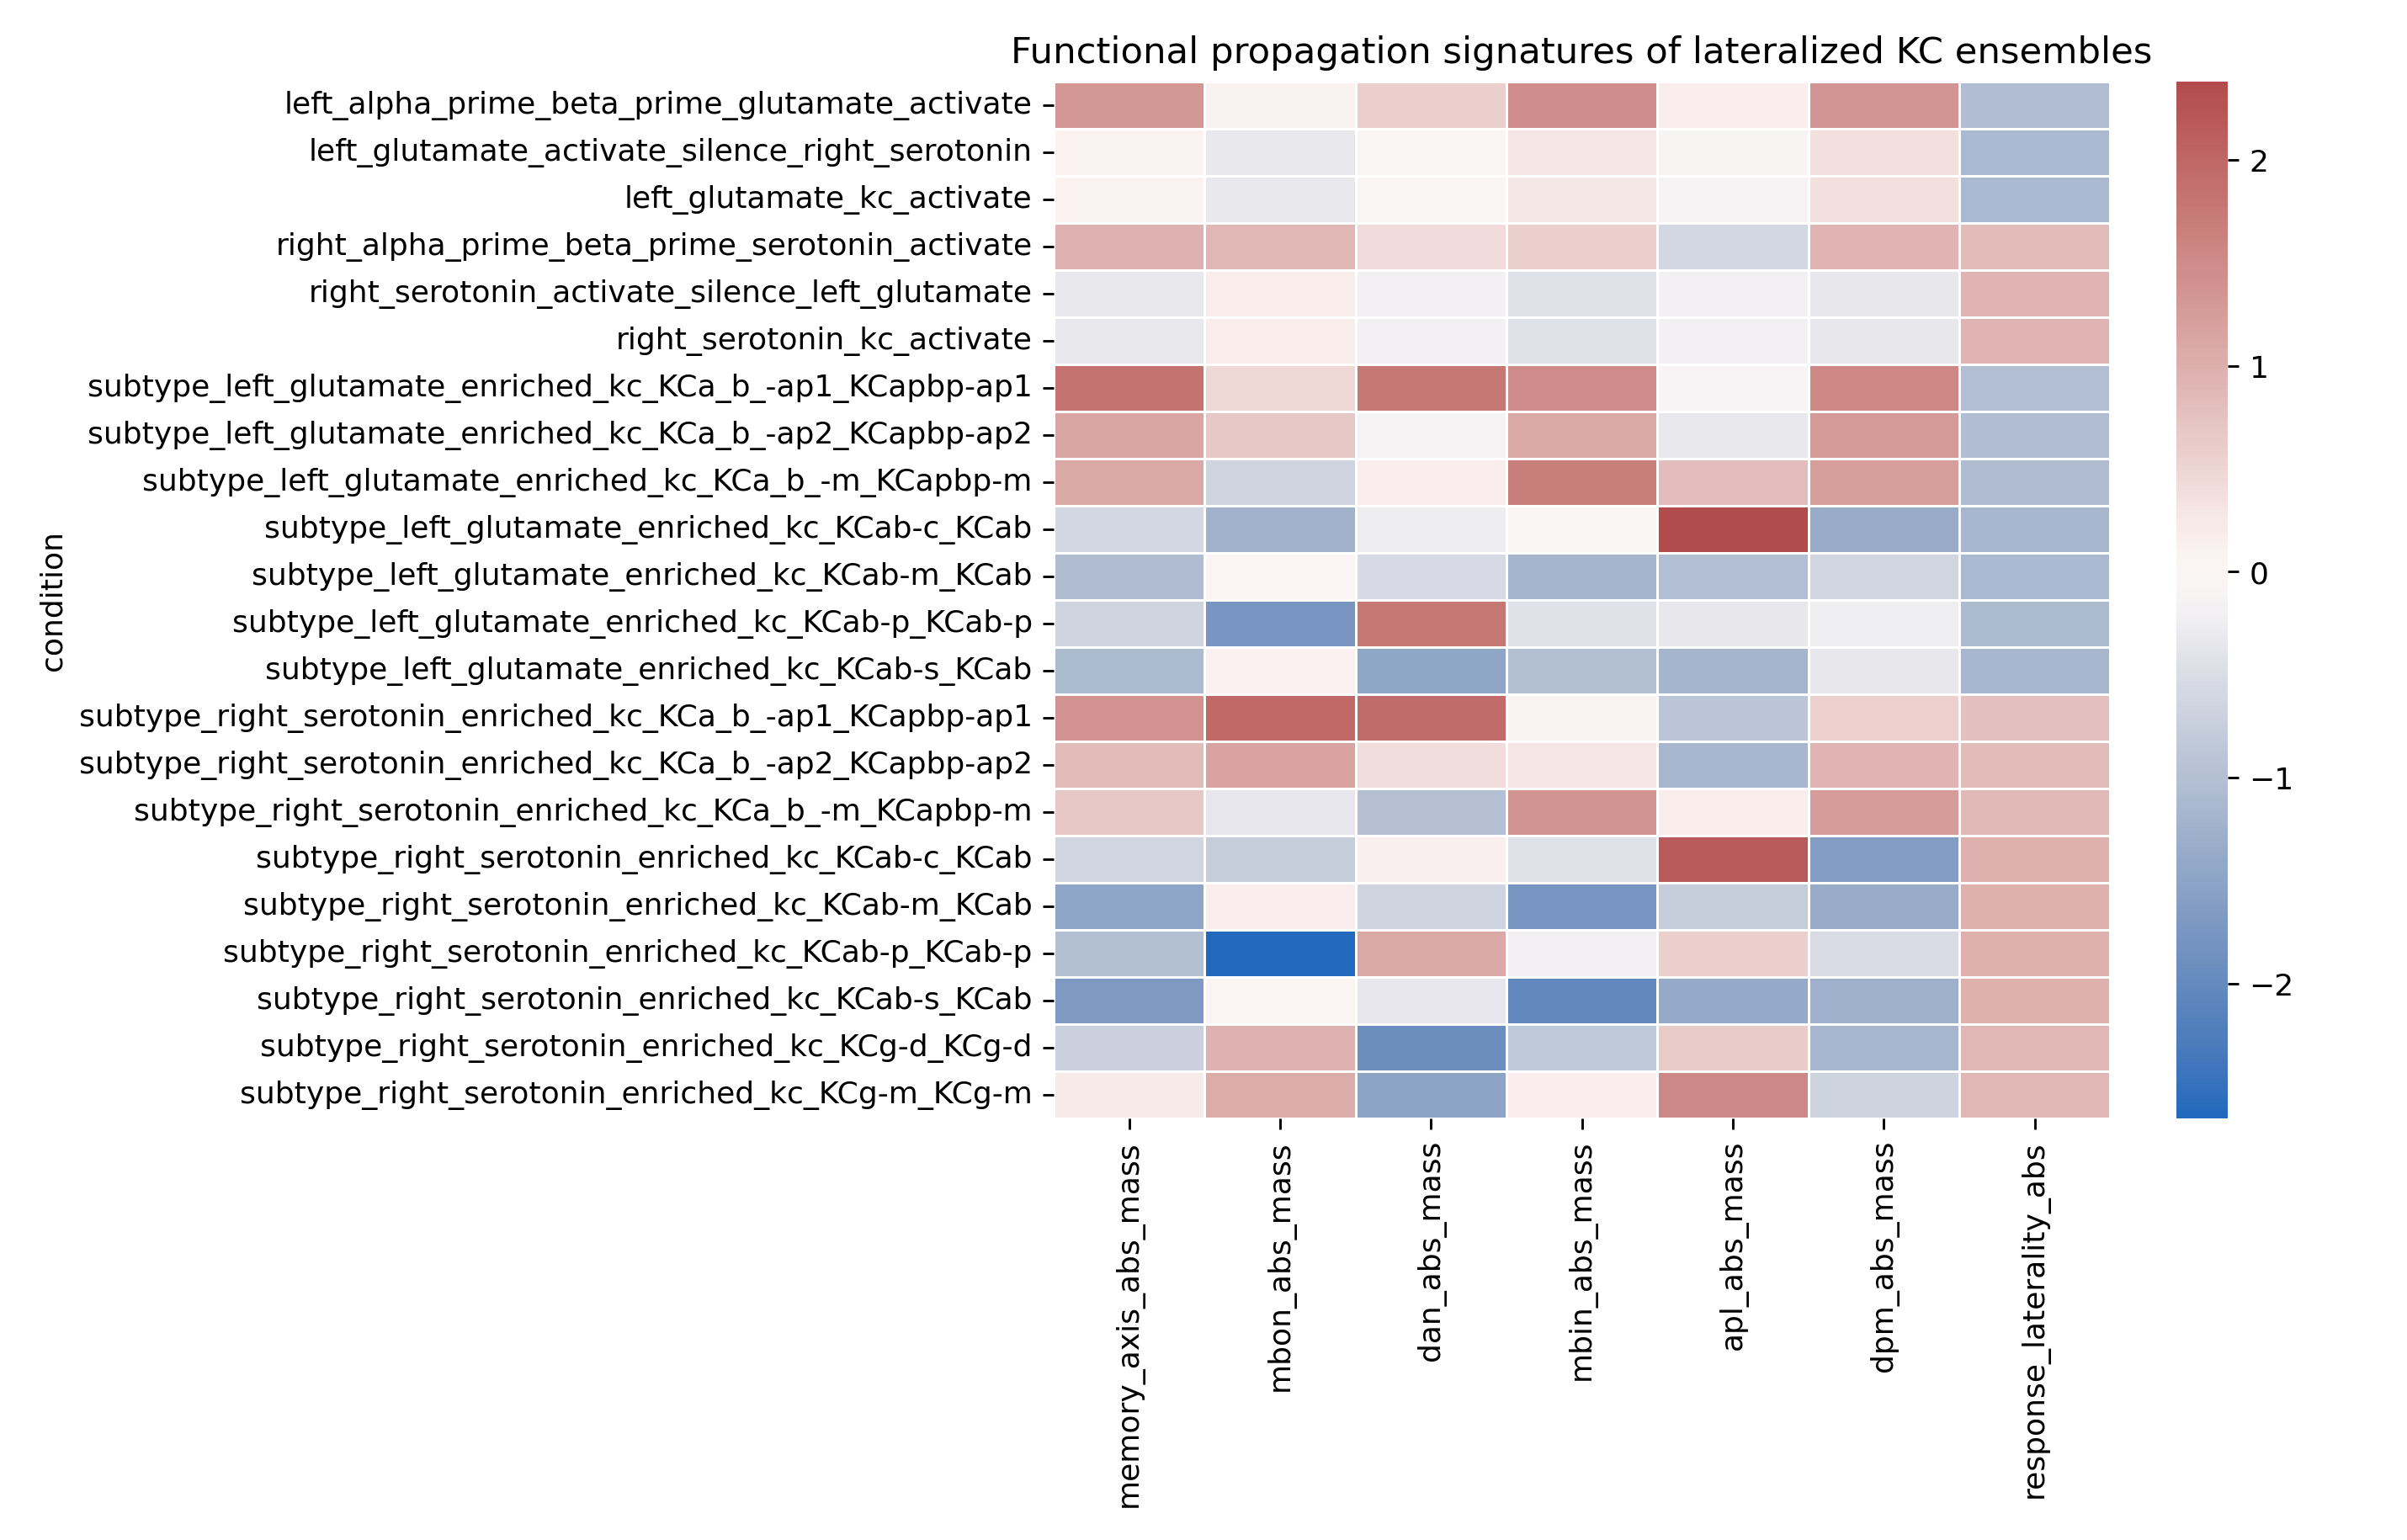
\includegraphics[width=0.63\linewidth]{figures/Fig2_functional_metric_heatmap.png}
\vspace{0.35em}
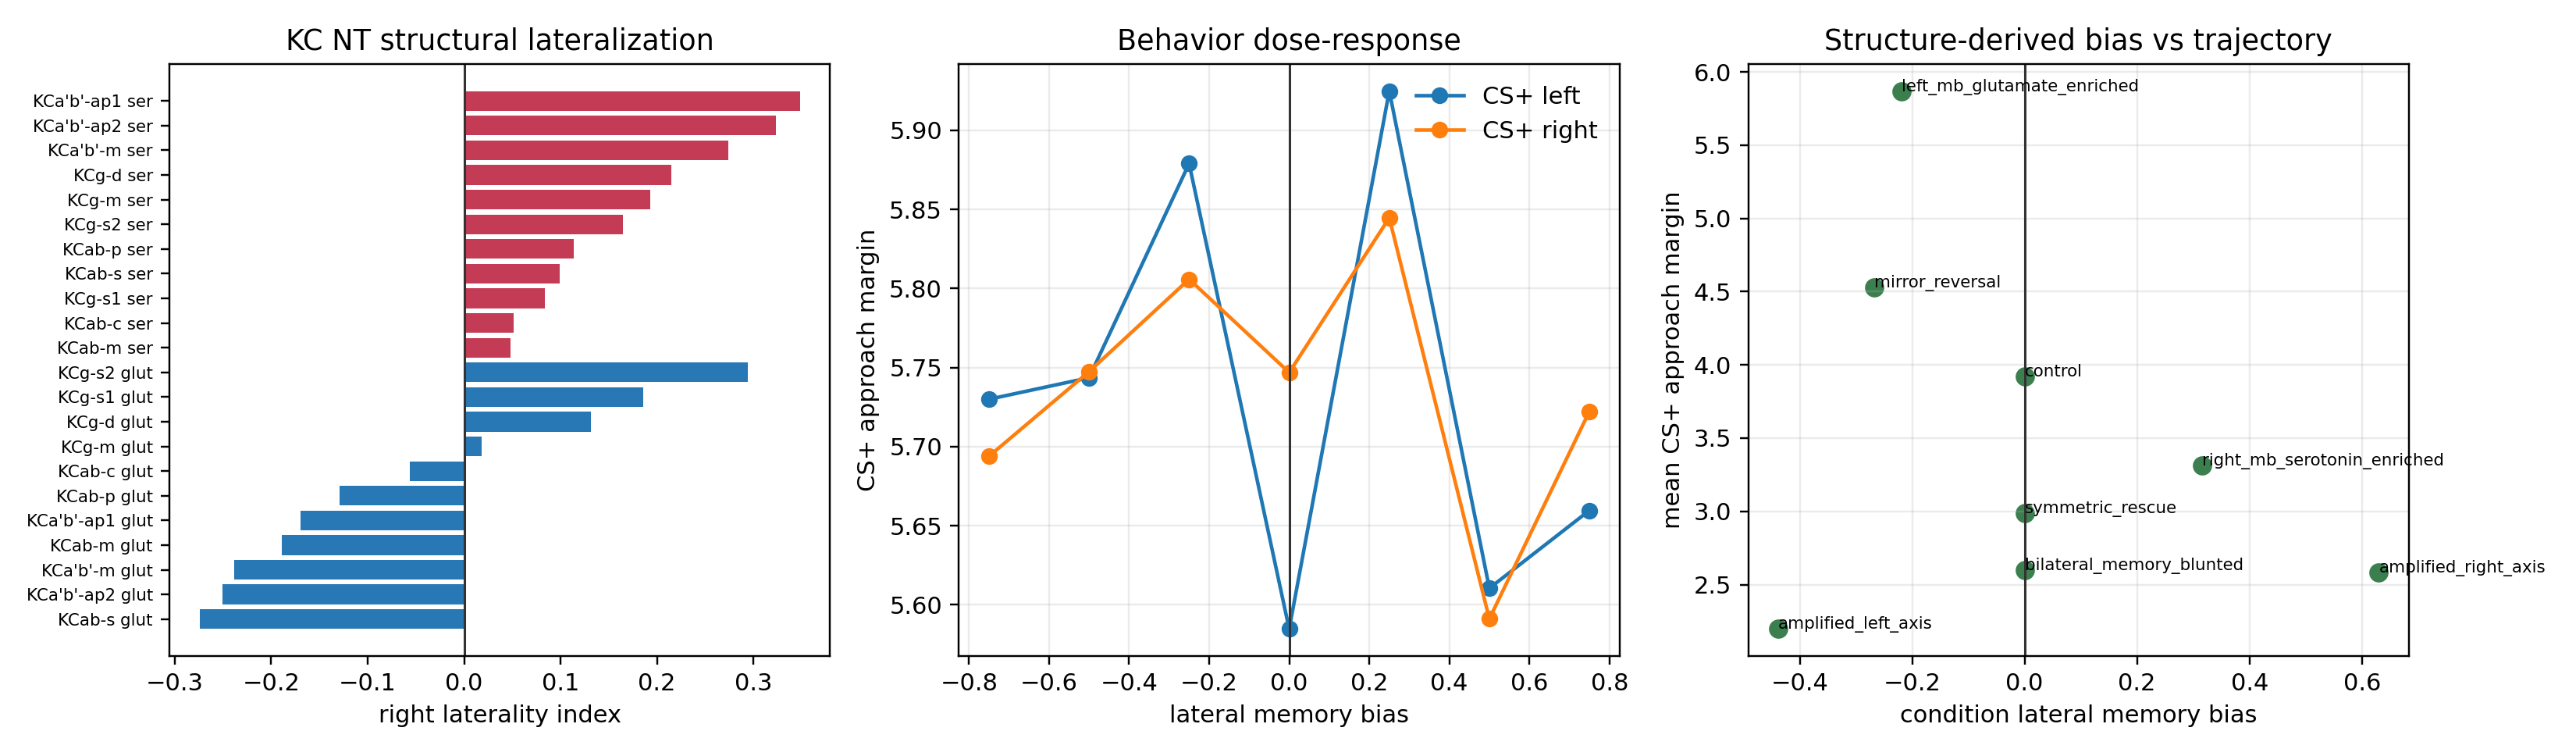
\includegraphics[width=0.49\linewidth]{figures/Fig_structure_behavior_linkage.png}
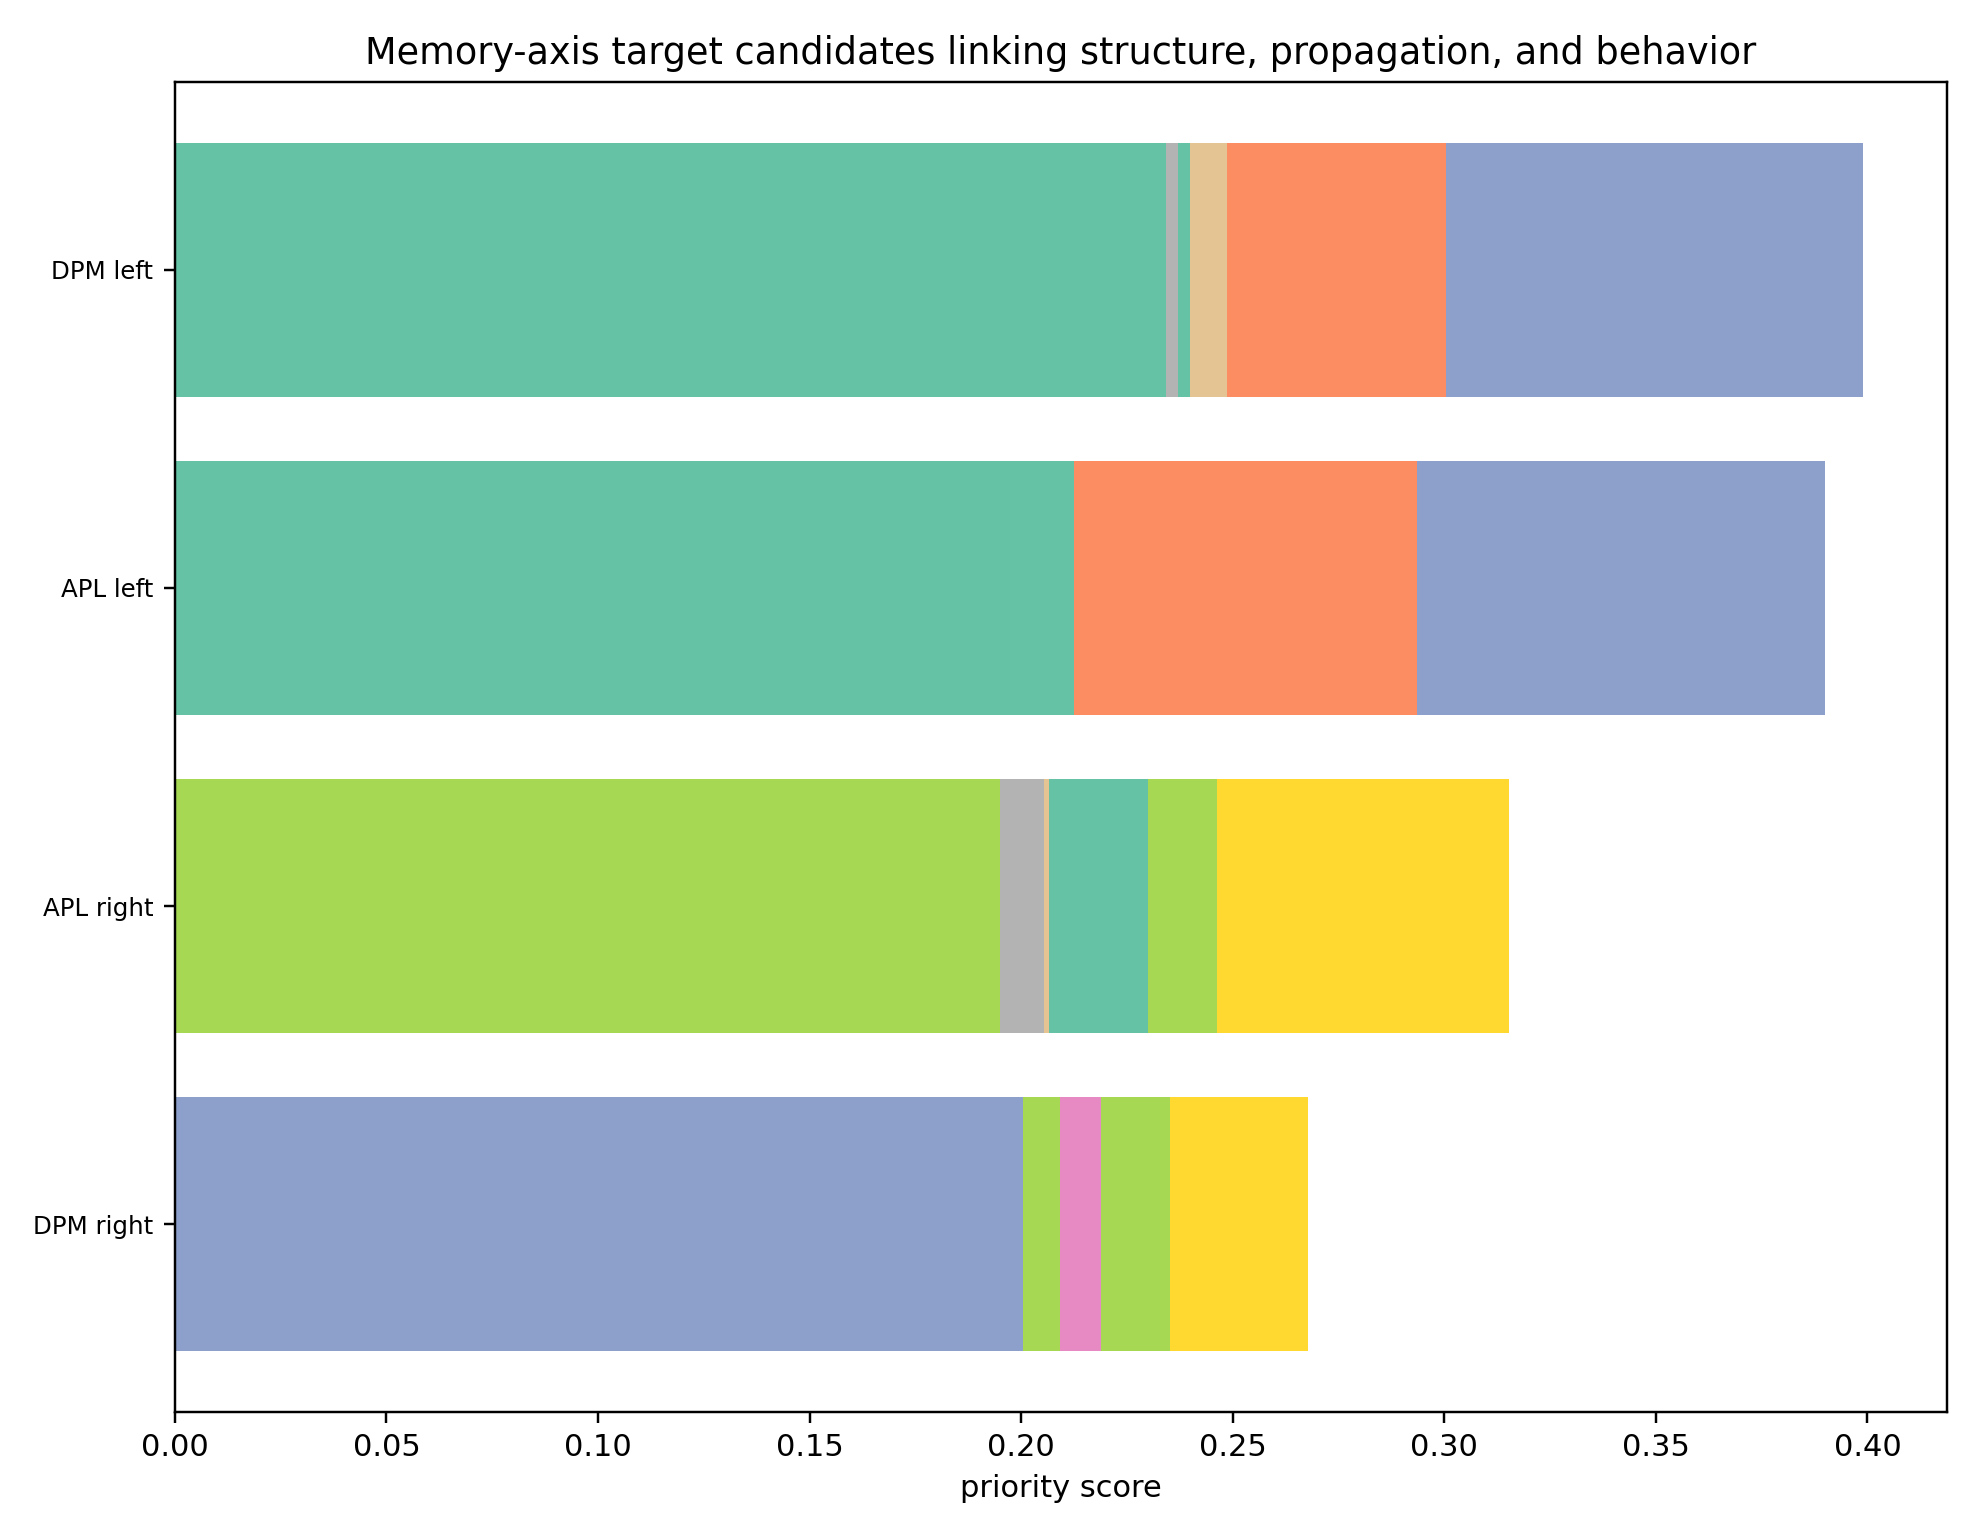
\includegraphics[width=0.49\linewidth]{figures/Fig_memory_axis_target_priorities.png}
\caption{\textbf{Functional bridge from structure to memory-circuit targets.}
\textbf{a}, The transmitter-selected KC ensembles do not behave like matched random controls: they recruit distinct memory-axis, DAN, APL, DPM and MBON/MBIN readouts.
\textbf{b}, The same propagation output can be translated into a concrete structure--behaviour linkage table.
\textbf{c}, Target-priority ranking highlights the MBON/DAN/APL/DPM families that should be retained for wet-lab follow-up rather than buried in a topology appendix.}
\label{fig:functional}
\end{figure}

% 中文注释：第三条结果是 DPM 与 OCT/MCH 验证。这里要把仿真、视频、湿实验之间的关系讲清楚，不能让人误以为视频本身就是证据。
\subsection*{DPM optogenetic surrogates yield wet-lab-ready predictions, and the weak-OCT/strong-MCH conflict assay is the most sensitive behaviour test}
The next question is how to translate this structural-functional chain into experiments. We chose DPM because it sits at the intersection of memory consolidation and 5-HT-related readout. We then scanned red-shifted optogenetic protocols for CsChrimson and ReaChR because these tools are more practical for adult fly validation than blue-light protocols that can introduce stronger visual confounds.

The protocol scan prioritizes 617--627 nm stimulation at 40 Hz, 20 ms pulse width and 5 s train duration, with low-to-moderate irradiance as the most informative starting point. Under the top protocols, the predicted DPM-driven 5-HT readout is right-biased after brain-side registration, with a laterality index around 0.80. The 180-degree rotation control is important here: if the asymmetry is real and brain-registered, rotating the fly should not change the sign; if the effect is only a camera-coordinate artifact, the sign will flip.

We then pushed the same readout into an OCT/MCH behavioural surrogate. The model identifies the weak-OCT/strong-MCH conflict condition as the best validation target because it avoids saturation and exposes lateralized memory competition. In that condition, the predicted choice-index shift is approximately +0.104 under the best DPM protocol. More ordinary appetitive and aversive conditions still move in the expected direction, but the conflict assay is the most sensitive test if the goal is to detect a modest behavioural bias in a group experiment.

% 中文注释：Figure 4 负责把验证逻辑收束到湿实验。右上角最好保留“旋转控制”，底部最好保留“弱冲突条件”。
\begin{figure}[!ht]
\centering
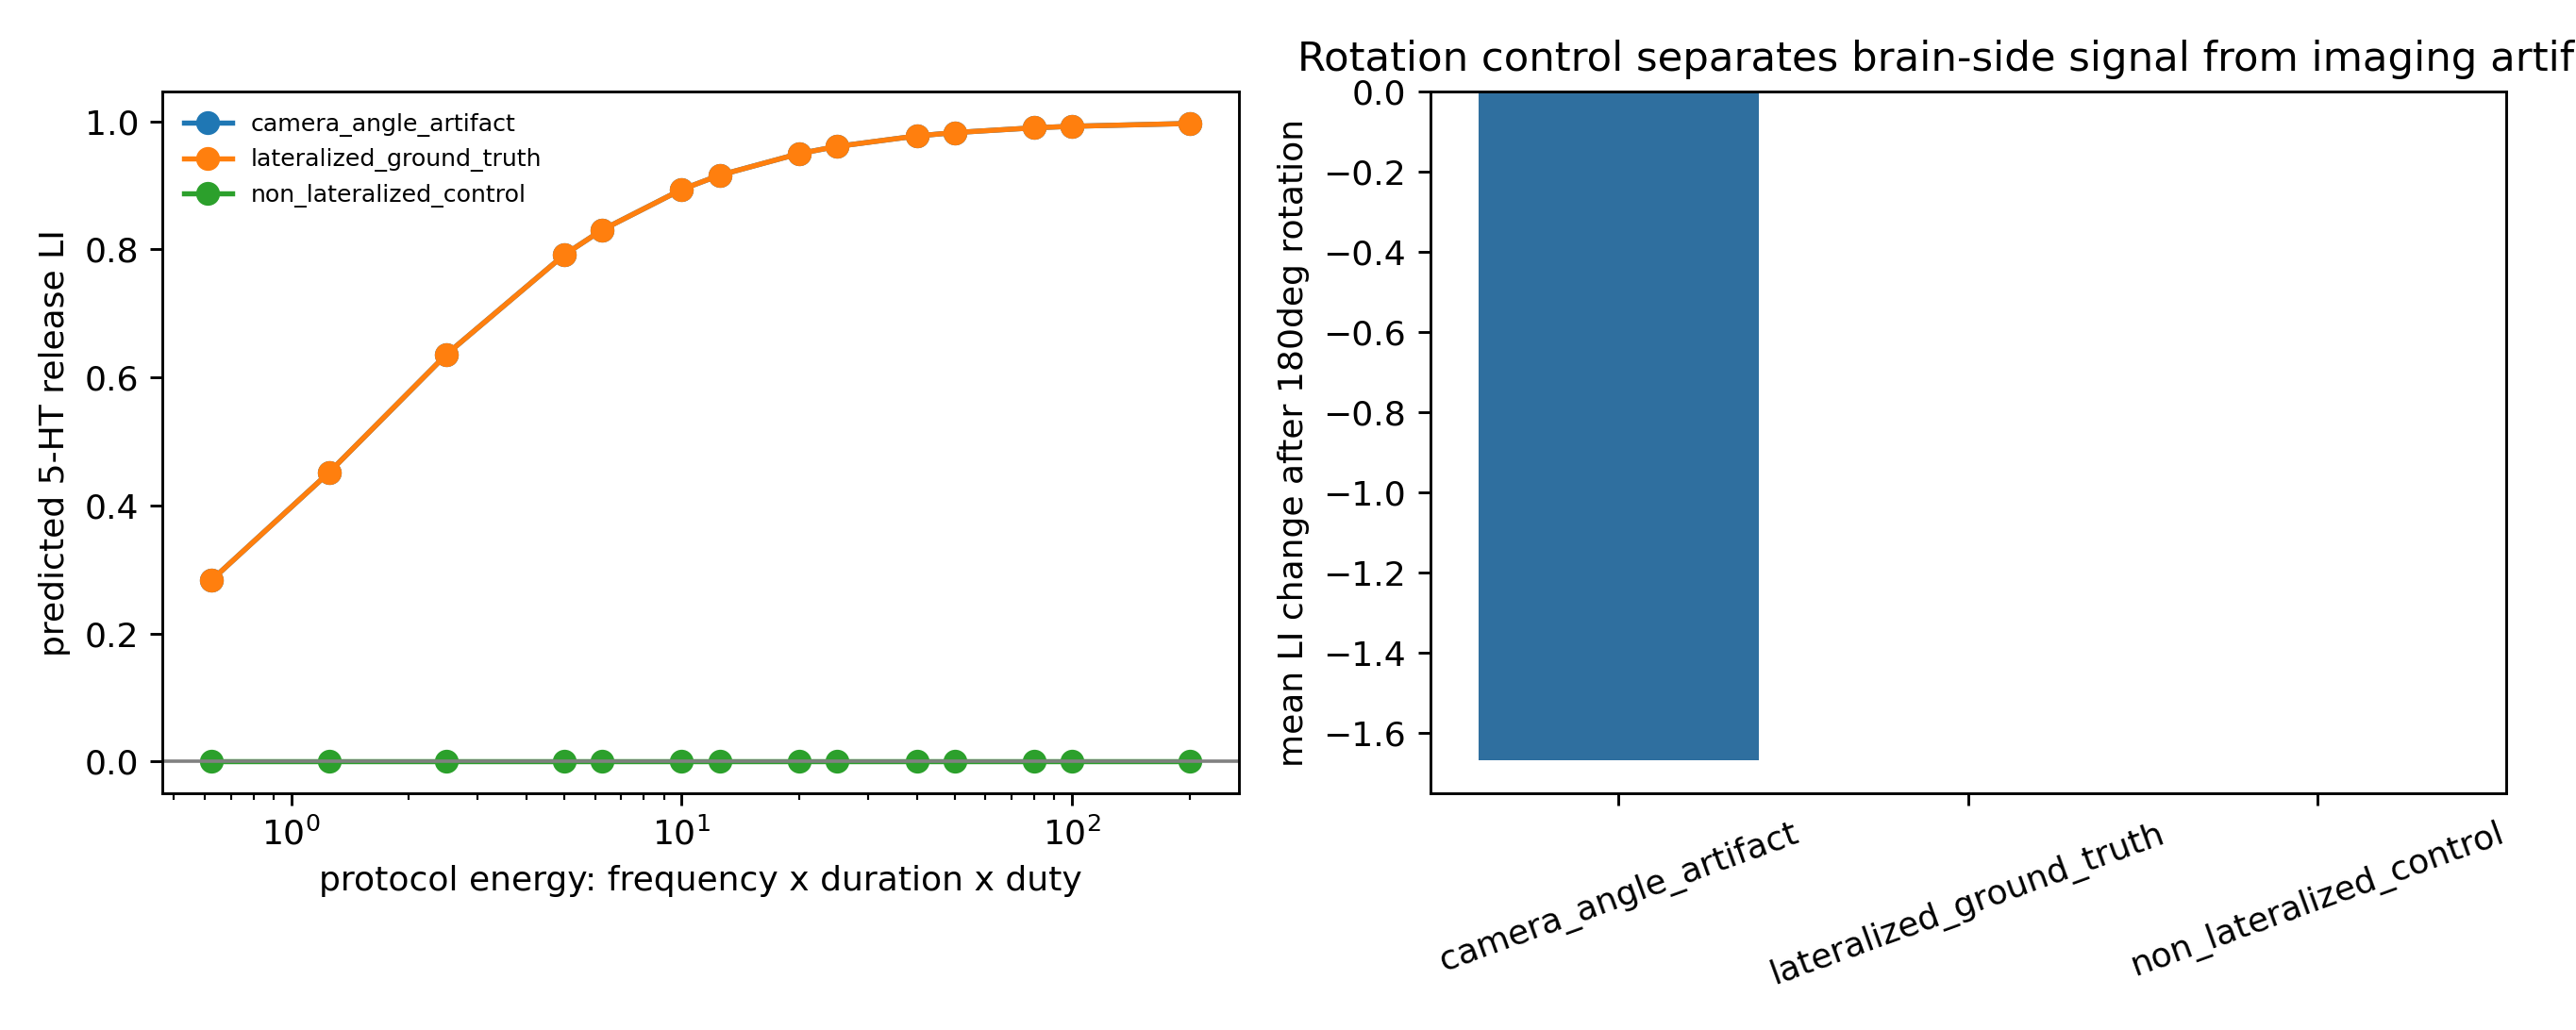
\includegraphics[width=0.49\linewidth]{figures/Fig_dpm_optogenetic_protocol_predictions.png}
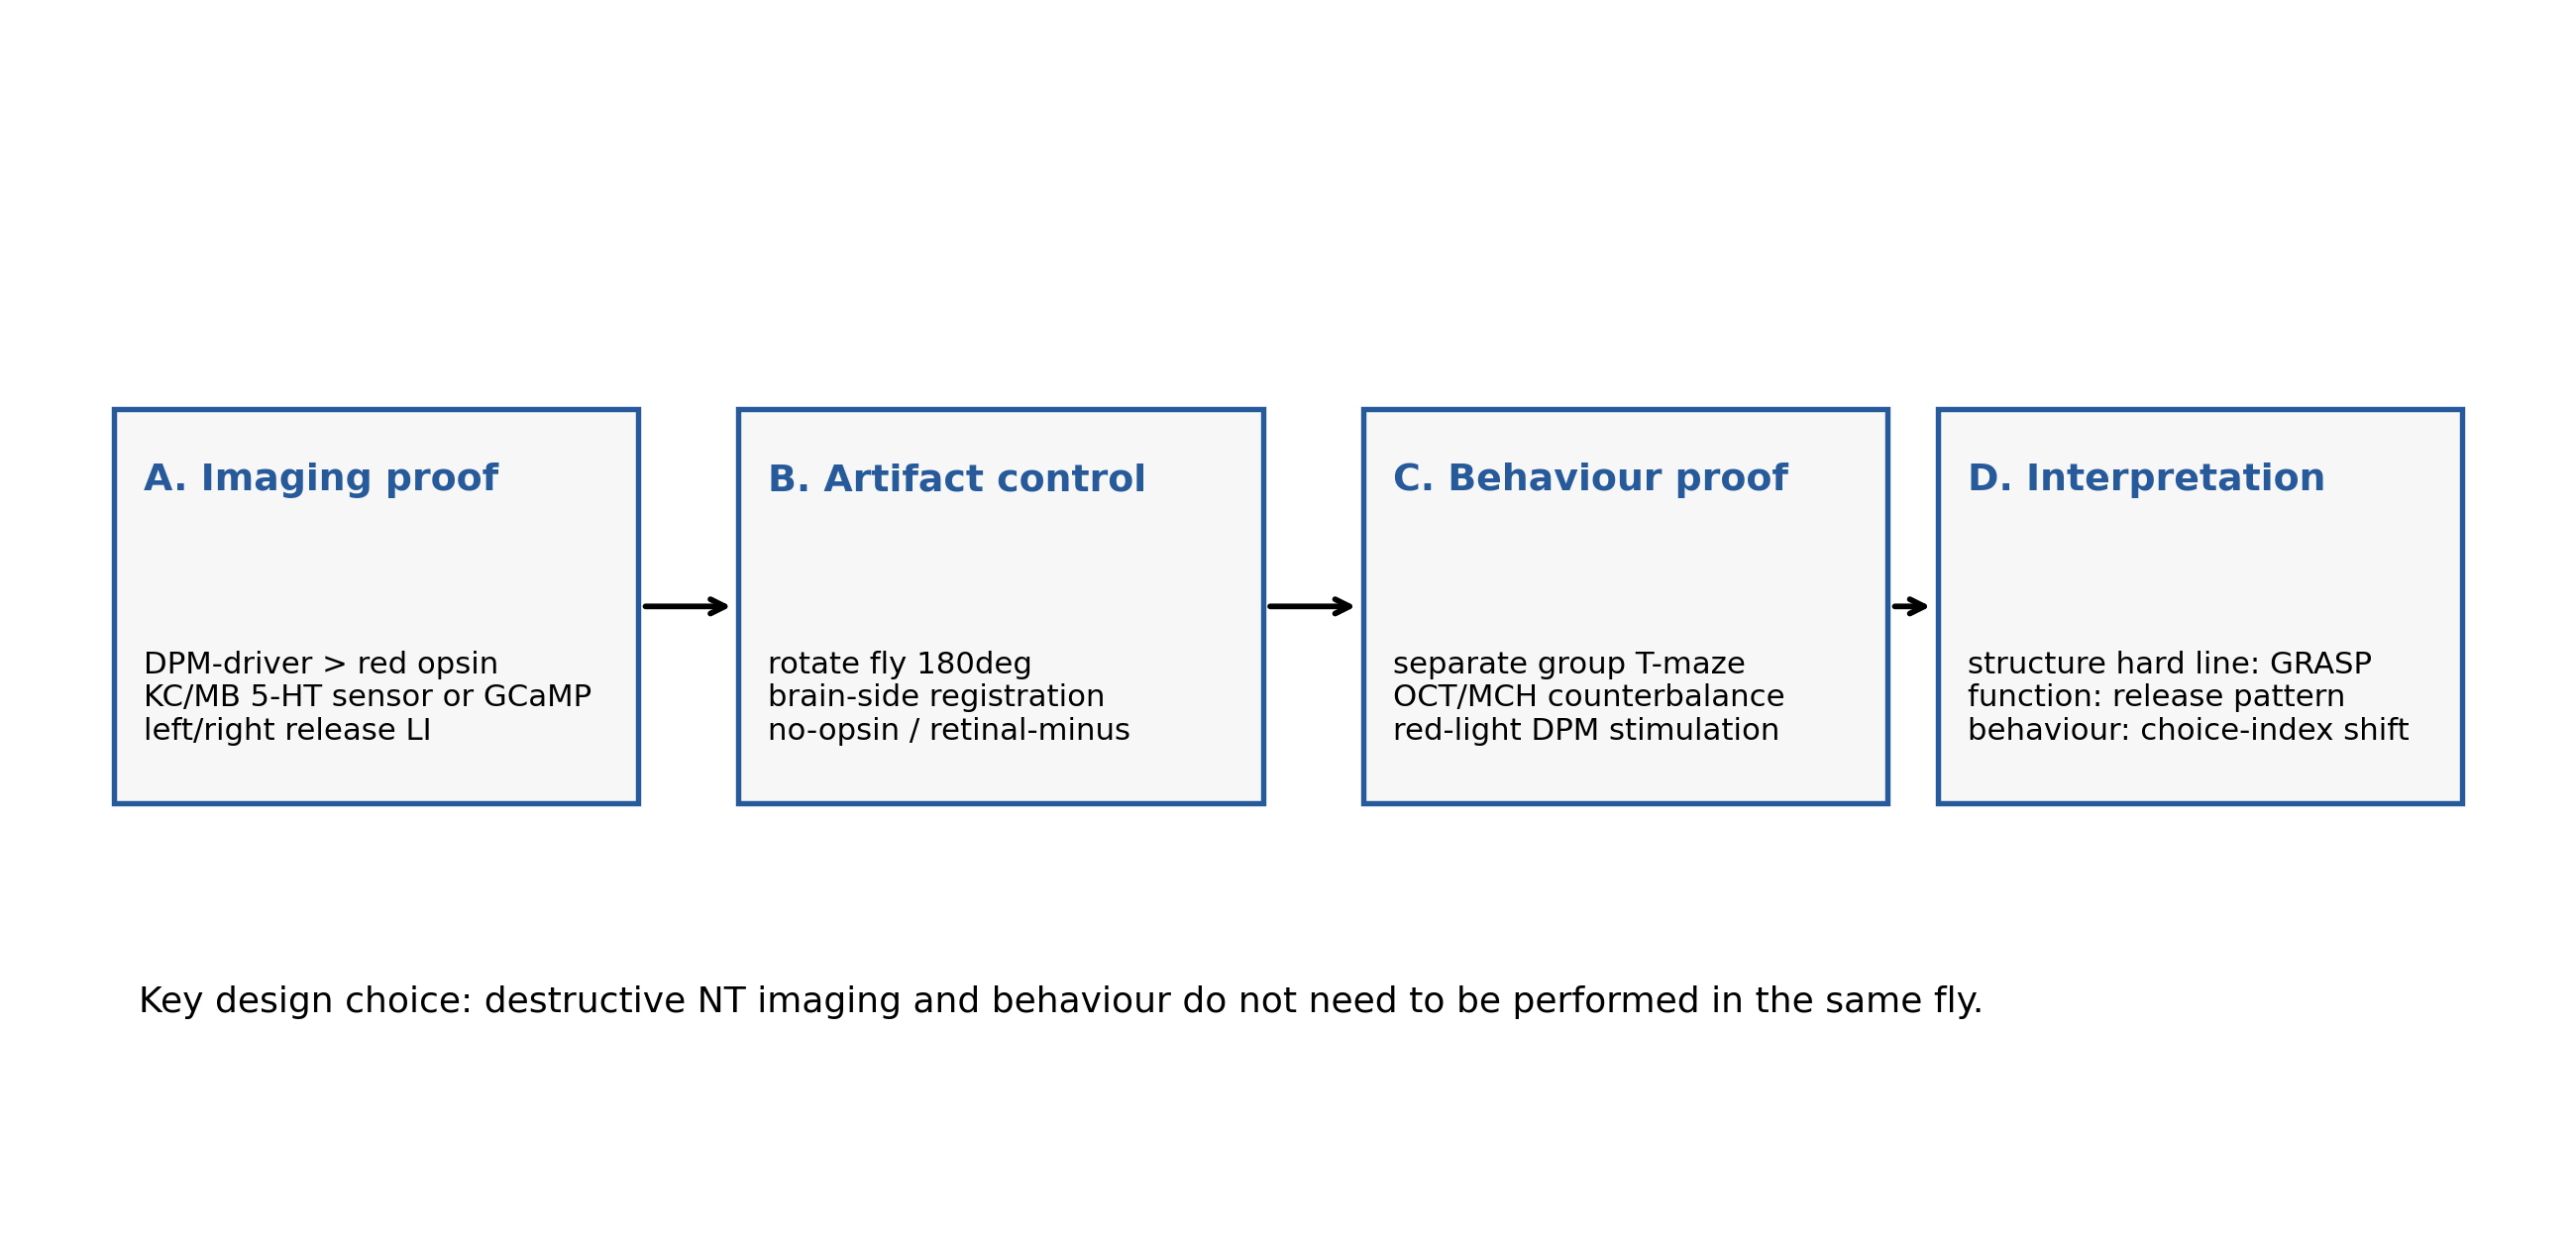
\includegraphics[width=0.49\linewidth]{figures/Fig_dpm_wetlab_validation_design.png}
\vspace{0.35em}
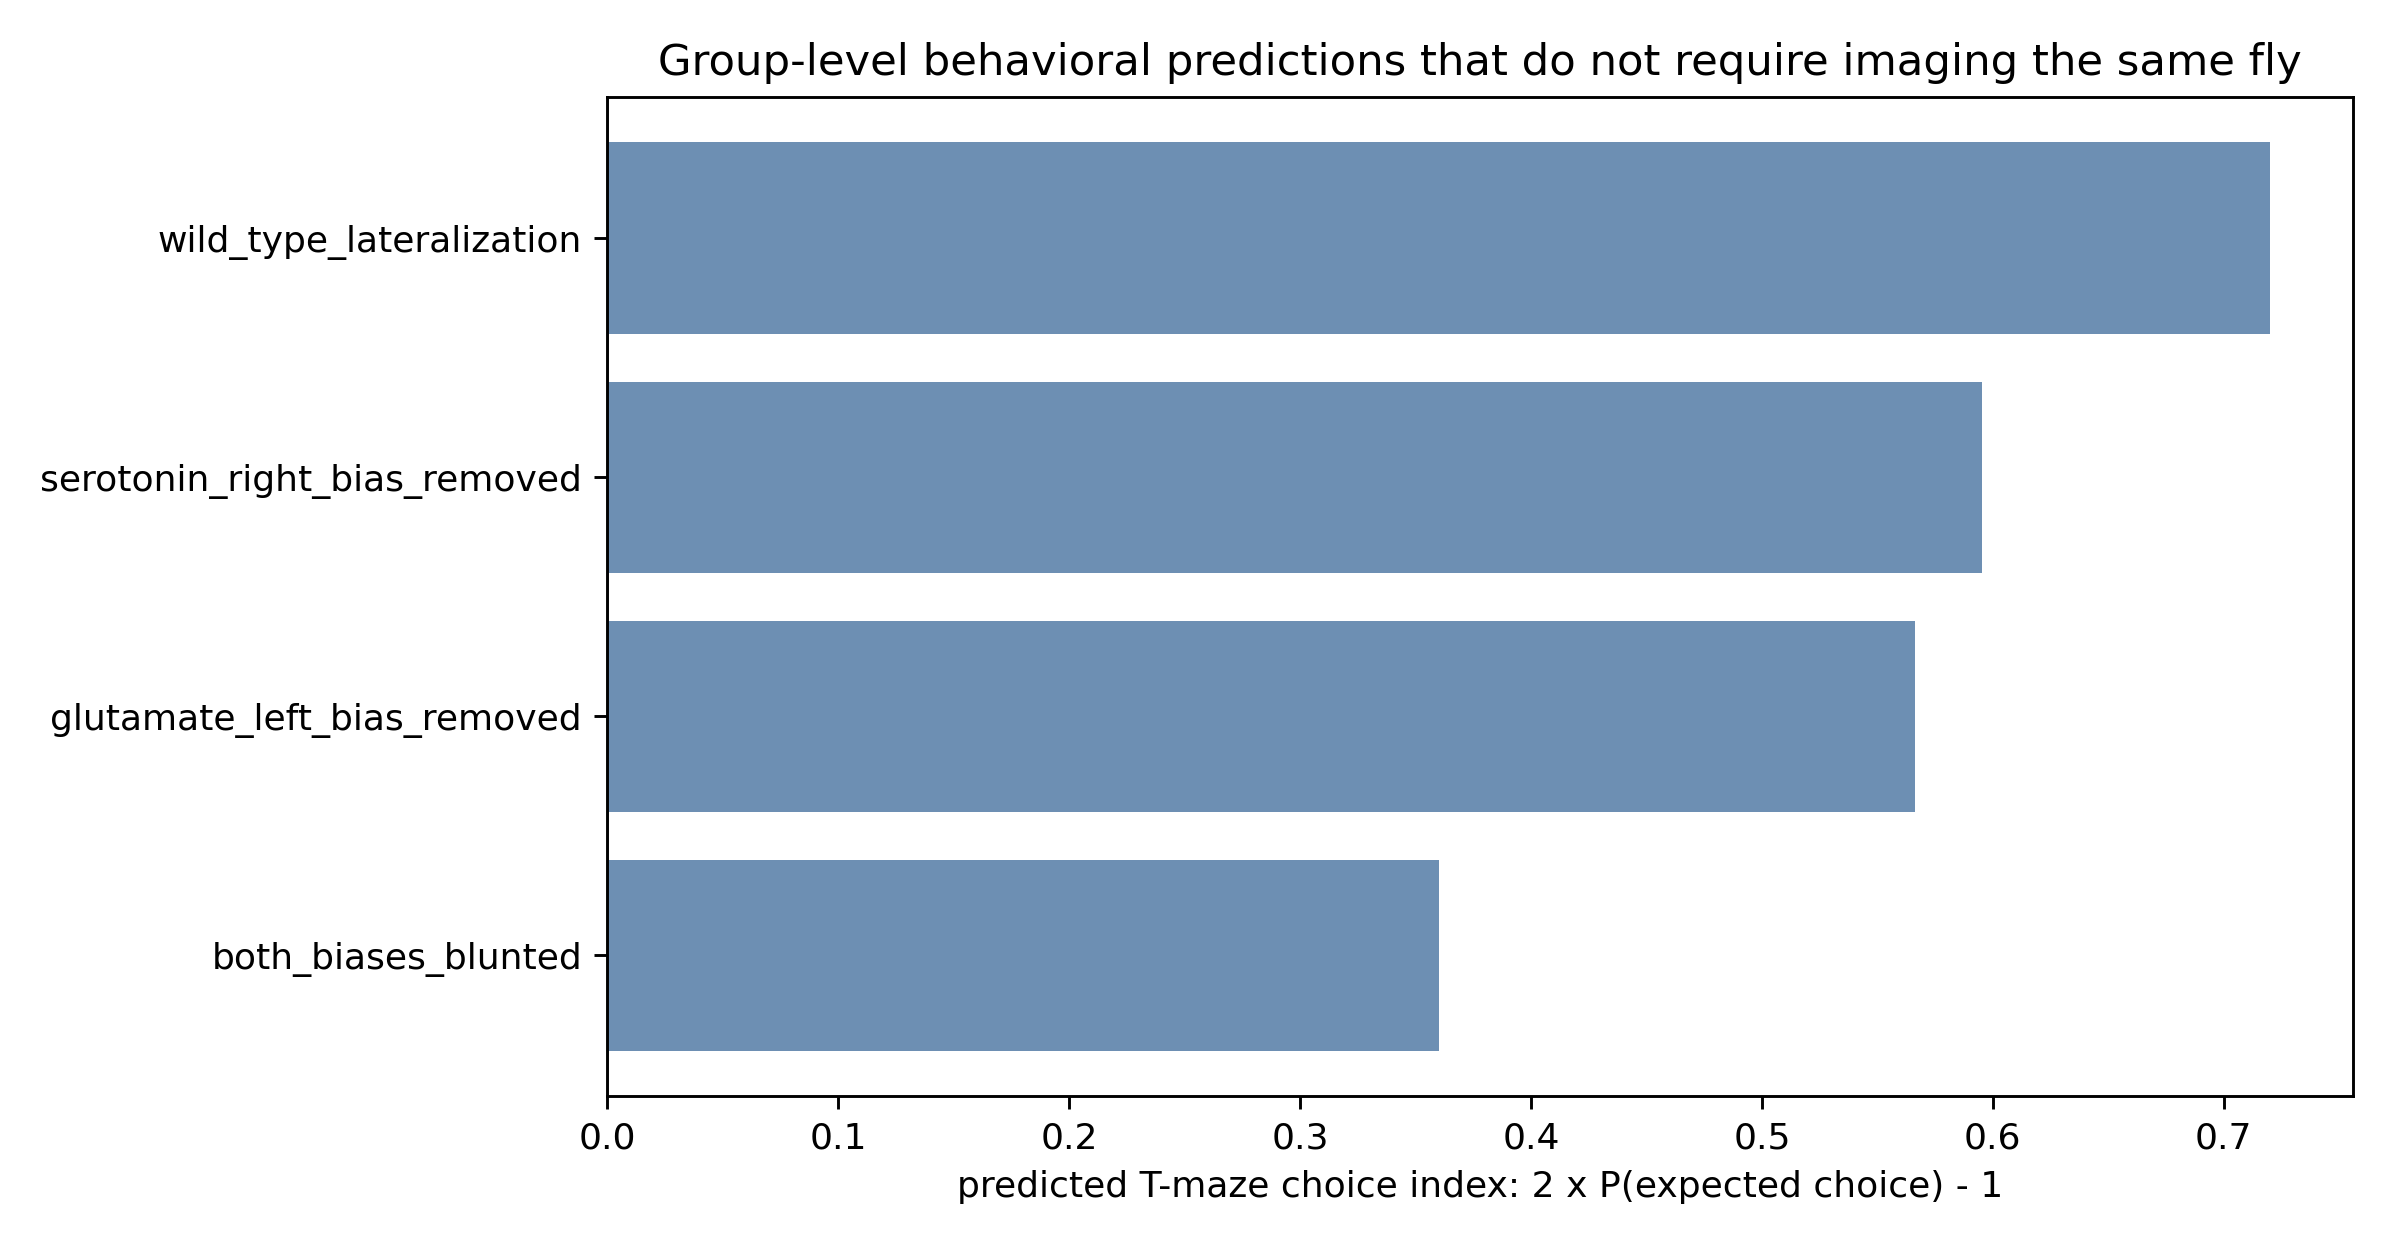
\includegraphics[width=0.49\linewidth]{figures/Fig_group_behavior_observable_predictions.png}
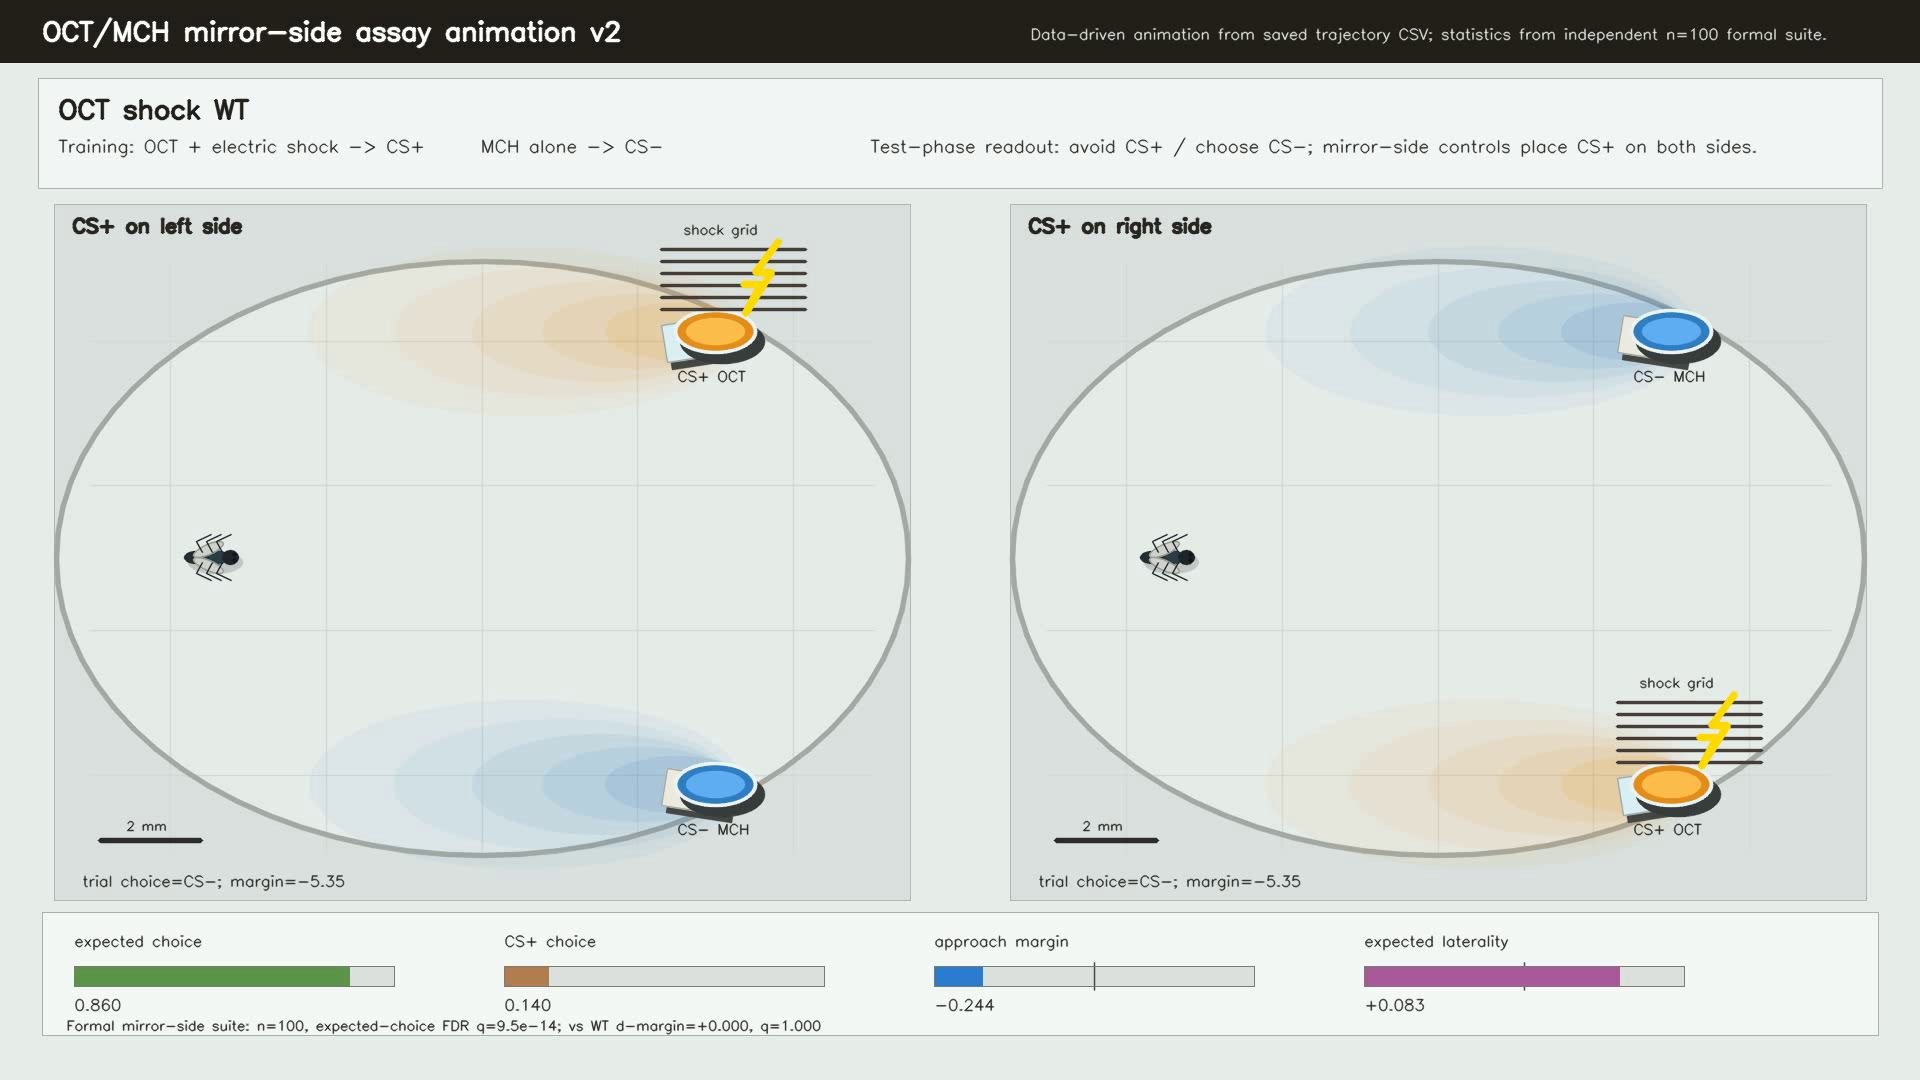
\includegraphics[width=0.49\linewidth]{figures/Fig_oct_mch_assay_v2_key_conditions_frame.png}
\caption{\textbf{DPM optogenetic and OCT/MCH validation path.}
\textbf{a}, The protocol scan prioritizes red-shifted CsChrimson/ReaChR stimulation.
\textbf{b}, The wet-lab design explicitly separates structural imaging from behaviour because the same individual cannot usually be used for both.
\textbf{c}, The behavioural proxy shows that the weak-OCT/strong-MCH conflict assay is the most sensitive group-level readout.
\textbf{d}, The representative assay frame gives the video a real experimental scene rather than a bare blue/yellow schematic.
Supplementary videos: \url{/unify/ydchen/unidit/bio_fly/paper/video/dpm_optogenetic_release_prediction.mp4} and \url{/unify/ydchen/unidit/bio_fly/paper/video/oct_mch_assay_v2_key_conditions.mp4}.}
\label{fig:dpm}
\end{figure}

% 中文注释：结论部分要明确“能说什么，不能说什么”，这也是 Nature 风格里最重要的部分之一。
\subsection*{What the current manuscript supports, and what it does not}
The strongest defensible conclusion is not that the connectome alone generates complete fly behaviour. The stronger and more accurate claim is that the adult fly MB contains a reproducible transmitter-level lateralization axis, that this axis is strongest in the memory-consolidation $\alpha'\beta'$ lobe, and that connectome-constrained propagation maps this axis onto memory-related readouts and experimentally actionable DPM/OCT-MCH validation routes.

Several things are therefore true at once. First, the structural signal is stable enough to survive multiple statistical checks. Second, the functional propagation is strong enough to separate transmitter-selected KC ensembles from matched random controls. Third, the behaviour surrogate is useful because it points to a concrete experimental design, not because it already proves the biology. Fourth, the manuscript still needs wet-lab follow-up: GRASP or split-GFP for structural contacts, DPM 5-HT or calcium imaging for functional readout, and group T-maze assays for behaviour.

% 中文注释：这一句给老师快速讲故事时可以直接引用。
\subsection*{Interpretation in one sentence}
The adult fly mushroom body is not just wired asymmetrically; it appears to use different transmitters on the two sides, and that chemical asymmetry is positioned to matter for memory.

\section*{Discussion}
This work is best read as a structure-to-function map. The structural side shows that the KC input channel is chemically lateralized. The functional side shows that the selected transmitter-defined ensembles propagate into memory-axis and feedback/output readouts rather than disappearing into generic connectome noise. The validation side shows how to turn that map into experiments without pretending that a public connectome has already solved full embodied behaviour.

That boundary is important. The current project deliberately stops short of claiming complete behaviour emergence from the connectome alone, and it does not claim that the public data fully reproduce a closed proprietary system. Instead, it identifies a tractable hypothesis: side-specific transmitter composition in KCs, strongest in $\alpha'\beta'$, may bias memory-related readout in a way that can be probed by DPM optogenetics and by group-level OCT/MCH assays.

\section*{Methods}
% 中文注释：方法只保留现在必须知道的部分，别再把拓扑表示学习放到主文里。拓扑/骨架相关内容以后只放补充或单独方法文档。
\subsection*{Data and computational setting}
All project data, scripts and outputs live under \url{/unify/ydchen/unidit/bio_fly}. The current environment is \url{/unify/ydchen/unidit/bio_fly/env}. GPU propagation jobs were run with explicit device assignment, typically \texttt{CUDA\_VISIBLE\_DEVICES=0,1}, to avoid interfering with other local jobs. The manuscript figures are drawn from the curated figure directory \url{/unify/ydchen/unidit/bio_fly/paper/figures}, and the behavioural and propagation tables reside in the corresponding \url{/unify/ydchen/unidit/bio_fly/outputs} subdirectories.

\subsection*{Structural analysis}
FlyWire v783 was used as the structural source of truth\cite{dorkenwald2024flywire,schlegel2024flywire}. Per-synapse neurotransmitter predictions were taken from the public classifier of Eckstein et al.\cite{eckstein2020neurotransmitter}. KC subtype labels were corrected so that $\alpha'\beta'$ types were not conflated with $\alpha\beta$ types. The primary statistic was Cohen's $d$ with an R--L sign convention. Secondary checks included Mann--Whitney tests, permutation tests, bootstrap confidence intervals and FDR correction.

\subsection*{Connectome propagation}
Selected KC seed ensembles were propagated through the signed FlyWire graph with a sparse GPU backend. Readouts were aggregated to memory-axis, DAN, APL, DPM, MBON and MBIN classes. Side-matched random KC ensembles with the same seed count served as null controls. The same propagation engine was then used for the DPM optogenetic surrogate and for the MB-to-DN interface summary.

\subsection*{Behavioural surrogate}
The OCT/MCH surrogate is a transparent rule-based model, not a trained end-to-end behaviour predictor. It converts DPM-driven release drive and laterality drive into choice-index deltas and approach margins. The weak-OCT/strong-MCH conflict condition is emphasized because it is the least saturated and therefore the most informative for a real experiment. Representative videos in \url{/unify/ydchen/unidit/bio_fly/paper/video} are visualizations of this surrogate and should be interpreted together with the formal statistics in the outputs directory.

\subsection*{What would count as wet-lab validation}
Structural validation should come from GRASP or split-GFP. Functional validation should come from DPM optogenetic imaging with a 180-degree rotation control and left/right brain registration. Behavioural validation should come from independent group T-maze tests in hundreds of flies. The current manuscript provides the quantitative priors for those experiments, not their final proof.

\section*{Data availability}
All paths below are absolute and are the current project locations used by the manuscript:
\begin{itemize}
  \item Main manuscript: \url{/unify/ydchen/unidit/bio_fly/paper/main_merged0601.tex}
  \item Structure statistics: \url{/unify/ydchen/unidit/bio_fly/outputs/kc_nt_lateralization/kc_nt_fraction_stats.csv}
  \item Functional propagation: \url{/unify/ydchen/unidit/bio_fly/outputs/four_card_suite/suite_empirical_significance.csv}
  \item Structure--behaviour linkage: \url{/unify/ydchen/unidit/bio_fly/outputs/structure_behavior_linkage/functional_behavior_linkage.csv}
  \item DPM optogenetic predictions: \url{/unify/ydchen/unidit/bio_fly/outputs/dpm_optogenetic_validation/tables/dpm_optogenetic_behavior_predictions.csv}
  \item OCT/MCH assay frame: \url{/unify/ydchen/unidit/bio_fly/paper/figures/Fig_oct_mch_assay_v2_key_conditions_frame.png}
  \item Supplementary video directory: \url{/unify/ydchen/unidit/bio_fly/paper/video}
\end{itemize}

\begin{thebibliography}{99}
\bibitem{deepwalk2014} Perozzi, B., Al-Rfou, R. \& Skiena, S. DeepWalk: Online learning of social representations. In \textit{Proc. KDD} 701--710 (2014).
\bibitem{node2vec2016} Grover, A. \& Leskovec, J. node2vec: Scalable feature learning for networks. In \textit{Proc. KDD} 855--864 (2016).
\bibitem{line2015} Tang, J., Qu, M., Wang, M., Zhang, M., Yan, J. \& Mei, Q. LINE: Large-scale information network embedding. In \textit{Proc. WWW} 1067--1077 (2015).
\bibitem{graphsage2017} Hamilton, W.L., Ying, Z. \& Leskovec, J. Inductive representation learning on large graphs. In \textit{Adv. Neural Inf. Process. Syst.} \textbf{30} (2017).
\bibitem{gcn2017} Kipf, T.N. \& Welling, M. Semi-supervised classification with graph convolutional networks. In \textit{ICLR} (2017).
\bibitem{gat2018} Veli\v{c}kovi\'c, P. et al. Graph attention networks. In \textit{ICLR} (2018).
\bibitem{rgcn2018} Schlichtkrull, M., Kipf, T.N., Bloem, P., van den Berg, R., Titov, I. \& Welling, M. Modeling relational data with graph convolutional networks. In \textit{The Semantic Web. ESWC 2018} 593--607 (Springer, 2018).
\bibitem{metapath2vec2017} Dong, Y., Chawla, N.V. \& Swami, A. metapath2vec: Scalable representation learning for heterogeneous networks. In \textit{Proc. KDD} (2017).
\bibitem{topoautoenc2020} Moor, M., Horn, M., Rieck, B. \& Borgwardt, K. Topological autoencoders. In \textit{Proc. ICML} 7045--7054 (2020).
\bibitem{perslay2020} Carri\`ere, M., Chazal, F., Ike, Y., Lacombe, T., Royer, M. \& Umeda, Y. PersLay: A neural network layer for persistence diagrams and new graph topological signatures. In \textit{Proc. AISTATS} 2786--2796 (2020).
\bibitem{scheffer2020hemibrain} Scheffer, L.K. et al. A connectome and analysis of the adult \textit{Drosophila} central brain. \textit{eLife} \textbf{9}, e57443 (2020).
\bibitem{li2020kc_subtypes} Li, F. et al. The connectome of the adult \textit{Drosophila} mushroom body provides insights into function. \textit{eLife} \textbf{9}, e62576 (2020).
\bibitem{costa2016nblast} Costa, M. et al. NBLAST: rapid, sensitive comparison of neuronal structure and construction of neuron family databases. \textit{Neuron} \textbf{91}, 293--311 (2016).
\bibitem{aso2014mushroom} Aso, Y. et al. The neuronal architecture of the mushroom body provides a logic for associative learning. \textit{eLife} \textbf{3}, e04577 (2014).
\bibitem{modi2020dopamine_kc} Modi, M.N. et al. The \textit{Drosophila} mushroom body: from architecture to algorithm in a learning circuit. \textit{Annu.\ Rev.\ Neurosci.} \textbf{43}, 465--484 (2020).
\bibitem{keene2006dpm} Keene, A.C. et al. \textit{Drosophila} dorsal paired medial neurons provide a general mechanism for memory consolidation. \textit{Curr.\ Biol.} \textbf{16}, 1524--1530 (2006).
\bibitem{waddell2013serotonin} Waddell, S. Reinforcement signalling in \textit{Drosophila}; dopamine does it all after all. \textit{Curr.\ Opin.\ Neurobiol.} \textbf{23}, 324--329 (2013).
\bibitem{karolis2019lateralisation} Karolis, V.R. et al. The architecture of functional lateralisation and its relationship to callosal connectivity in the human brain. \textit{Nat.\ Commun.} \textbf{10}, 1417 (2019).
\bibitem{pedigo2023bilateral_elife} Pedigo, B.D. et al. Bisected graph matching improves automated pairing of bilaterally homologous neurons from connectomes. \textit{eLife} \textbf{12}, e80664 (2023).
\bibitem{winding2023larva} Winding, M. et al. The connectome of an insect brain. \textit{Science} \textbf{379}, eadd9330 (2023).
\bibitem{pascual2004lateralized} Pascual, A. et al. Localization of long-term memory within the \textit{Drosophila} mushroom body. \textit{Science} \textbf{304}, 1024--1027 (2004).
\bibitem{dorkenwald2024flywire} Dorkenwald, S. et al. Neuronal wiring diagram of an adult brain. \textit{Nature} \textbf{634}, 124--138 (2024).
\bibitem{schlegel2024flywire} Schlegel, P. et al. Whole-brain annotation and multi-connectome cell typing of \textit{Drosophila}. \textit{Nature} \textbf{634}, 139--152 (2024).
\bibitem{eckstein2020neurotransmitter} Eckstein, N. et al. Neurotransmitter classification from electron microscopy images at synaptic sites in \textit{Drosophila melanogaster}. \textit{Cell} \textbf{187}, 2574--2594 (2024).
\end{thebibliography}

\end{document}
